% ============================================== %
% Author: Lucian Dorin Crainic <https://luciancrainic.github.io/>
%
% Thesis Title: TODO
%
% Master of Science in Computer Science, Sapienza University of Rome.
%
% https://github.com/LucianCrainic/MSc-Thesis/
%
% Build from the repository root with:
%   inv thesis
%
% ============================================== %

% Document Class
\documentclass[binding=0.6cm]{sapthesis}

% Packages
\usepackage{microtype}
\usepackage[english]{babel}
\usepackage[T1]{fontenc}
\usepackage{hyperref}
\usepackage{listings}
\usepackage{xcolor}
\usepackage{geometry} 
\usepackage{caption}  
\usepackage[edges]{forest}
\usepackage{subcaption}
\usepackage{float}    
\usepackage{lipsum}  
\usepackage{xargs}                     
\usepackage{booktabs}
\usepackage{graphicx}
\usepackage{makecell}
\usepackage{tabularx}
\usepackage{xltabular}
\usepackage{longtable}
\usepackage{threeparttable}
\usepackage{amsmath}
\usepackage{amssymb}
\usepackage{array}
\usepackage{enumitem}
\usepackage{colortbl}
\usepackage{flafter}
\usepackage{placeins}
\usepackage{tikz}
\usetikzlibrary{arrows.meta, positioning, fit, calc}
\usepackage{xurl}
\usepackage[numbers,sort&compress]{natbib}
\usepackage[colorinlistoftodos,prependcaption,textsize=tiny]{todonotes}

% Commands and Settings
\newcommandx{\unsure}[2][1=]{\todo[linecolor=red,backgroundcolor=red!25,bordercolor=red,#1]{#2}}
\newcommandx{\change}[2][1=]{\todo[linecolor=blue,backgroundcolor=blue!25,bordercolor=blue,#1]{#2}}
\newcommandx{\info}[2][1=]{\todo[linecolor=OliveGreen,backgroundcolor=OliveGreen!25,bordercolor=OliveGreen,#1]{#2}}
\newcommandx{\improvement}[2][1=]{\todo[linecolor=Plum,backgroundcolor=Plum!25,bordercolor=Plum,#1]{#2}}
\newcommandx{\thiswillnotshow}[2][1=]{\todo[disable,#1]{#2}}
\newcolumntype{L}[1]{>{\raggedright\arraybackslash}p{#1}}
\newcolumntype{Y}{>{\raggedright\arraybackslash}X}
\newcolumntype{P}[1]{>{\raggedright\arraybackslash}p{#1}}
\graphicspath{{figures/}}

\definecolor{accent}{RGB}{128,0,32}
\definecolor{hbmcol}{RGB}{213,125,28}
\definecolor{ddrcol}{RGB}{55,105,165}
\definecolor{neutralcol}{RGB}{235,238,242}
\definecolor{citecol}{RGB}{128,0,32}
% Match the Sapienza burgundy used by sapthesis on the title page.
\definecolor{figcol}{RGB}{130,36,51}
\definecolor{tabcol}{RGB}{35,82,145}
\definecolor{eqcol}{RGB}{112,54,132}
\definecolor{seccol}{RGB}{85,85,95}
% Tables share the flat Sapienza red used in the drawings.
\colorlet{tabhead}{figcol}
\definecolor{tabstripe}{HTML}{F2F4F6}
\definecolor{tabline}{HTML}{D8DEE5}

\setlist[itemize]{leftmargin=*, itemsep=2pt, topsep=4pt}
\setlist[enumerate]{leftmargin=*, itemsep=2pt, topsep=4pt}
\captionsetup{font=small, labelfont=bf}
\captionsetup[figure]{labelfont={bf,color=figcol}}
\captionsetup[table]{position=bottom, skip=8pt, labelfont={bf,color=tabcol}}
\setlength{\emergencystretch}{2.5em}
\widowpenalty=10000
\clubpenalty=10000
\raggedbottom
\setcounter{topnumber}{3}
\setcounter{bottomnumber}{2}
\setcounter{totalnumber}{4}
\renewcommand{\topfraction}{0.9}
\renewcommand{\bottomfraction}{0.7}
\renewcommand{\textfraction}{0.07}
\renewcommand{\floatpagefraction}{0.75}
\setlength{\textfloatsep}{14pt plus 3pt minus 3pt}
\setlength{\intextsep}{13pt plus 3pt minus 3pt}

\newcommand{\figref}[1]{\hyperref[#1]{\textcolor{figcol}{Figure~\ref*{#1}}}}
\newcommand{\tabref}[1]{\hyperref[#1]{\textcolor{tabcol}{Table~\ref*{#1}}}}
\newcommand{\eqnref}[1]{\hyperref[#1]{\textcolor{eqcol}{Equation~\ref*{#1}}}}
\newcommand{\secref}[1]{\hyperref[#1]{\textcolor{seccol}{Section~\ref*{#1}}}}
\newcommand{\chapref}[1]{\hyperref[#1]{\textcolor{seccol}{Chapter~\ref*{#1}}}}
\newcommand{\eqcaption}[1]{%
  \par\vspace{-2pt}%
  \begingroup
    \small
    \setlength{\baselineskip}{12.5pt}%
    \noindent\textcolor{eqcol}{\textbf{Equation~\theequation:}}~#1\par
  \endgroup
  \vspace{9pt}}
\newcommand{\headrow}{\rowcolor{tabhead}}
\newcommand{\headcell}[1]{\textcolor{white}{\textbf{#1}}}
\newcommand{\tabstripeRow}{\rowcolor{tabstripe}}
\newcommand{\tabplainRow}{\rowcolor{white}}
\newcommand{\tabrowsep}{\arrayrulecolor{tabline}\hline}
\newcommand{\tabheadrule}{\arrayrulecolor{white}\hline\arrayrulecolor{tabline}}
\newcommand{\tabbottomrule}{\arrayrulecolor{tabhead}\hline\arrayrulecolor{tabline}}
% Keep these settings local to each table or grouped multipage table.
% Explicit body-row colours preserve the stripe sequence across page breaks.
\newcommand{\tabsetup}{%
  \renewcommand{\arraystretch}{1.18}%
  \setlength{\tabcolsep}{6pt}%
  \setlength{\extrarowheight}{3pt}%
  \setlength{\arrayrulewidth}{0.35pt}%
  \arrayrulecolor{tabline}}
\newcommand{\lcpp}{\texttt{llama.cpp}}
\newcommand{\ggml}{\texttt{ggml}}
\newcounter{boxlblcounter}  
\newcommand{\makeboxlabel}[1]{\fbox{#1.}\hfill}
\newenvironment{boxlabel}
  {\begin{list}
    {\arabic{boxlblcounter}}
    {\usecounter{boxlblcounter}
     \setlength{\labelwidth}{3em}
     \setlength{\labelsep}{0em}
     \setlength{\itemsep}{2pt}
     \setlength{\leftmargin}{1.5cm}
     \setlength{\rightmargin}{2cm}
     \setlength{\itemindent}{0em} 
     \let\makelabel=\makeboxlabel
    }
  }
{\end{list}}
\lstdefinestyle{myStyle}{
    belowcaptionskip=1\baselineskip,
    breaklines=true,
    numbers=left,
    numberstyle=\tiny\color{gray},
    captionpos=t,
    frame=lines,
    basicstyle=\footnotesize\ttfamily,
    prebreak=\raisebox{0ex}[0ex][0ex]{\ensuremath{\hookleftarrow}},
    keywordstyle=\bfseries\color{green!60!black},
    commentstyle=\itshape\color{blue!40!black},
    identifierstyle=\color{black},
    backgroundcolor=\color{white},
}
\lstset{style=mystyle}
\lstdefinestyle{shell}{
    language=bash,
    basicstyle=\ttfamily\footnotesize,
    backgroundcolor=\color{neutralcol},
    frame=single,
    rulecolor=\color{black!25},
    framerule=0.4pt,
    columns=fullflexible,
    keepspaces=true,
    breaklines=true,
    showstringspaces=false,
    aboveskip=8pt,
    belowskip=8pt,
}

% Metadata
\hypersetup{pdftitle={Thesis},pdfauthor={Lucian Dorin Crainic}, urlcolor=black, linkcolor=black, citecolor=citecol, colorlinks=true}
\title{TODO}
\author{Lucian Dorin Crainic}
\IDnumber{1938430}
\course{Master's Degree in Computer Science}
\courseorganizer{Faculty of Information Engineering, Computer Science and Statistics}
\AcademicYear{2026/2027}
\advisor{Prof. Salvatore Pontarelli}
\coadvisor{Prof. Daniele De Sensi\\[1mm]Dr. Marco Faltelli}
\authoremail{crainic.lucian@gmail.com}
\copyyear{20xx}
\thesistype{Master's Thesis}

% ================== DOCUMENT ==================
\begin{document}

\lstset{language=Python}

\frontmatter

\maketitle

% ================== QUOTATION ==================
\dedication{% Source: https://medium.com/@myqitraining/i-loved-every-minute-of-it-no-matter-how-hard-it-had-been-4f9da196738f
\begin{minipage}{0.72\textwidth}
    \raggedright
    {\Large\itshape
    ``I loved every minute of it,\\[0.25em]
    no matter how hard it had been.''\par}
    \vspace{1.4em}
    {\raggedleft
    \textcolor{accent}{\rule{2.2em}{0.5pt}}\par
    \vspace{0.6em}
    \normalfont\small\textsc{Sir Andrew Wiles}\par}
\end{minipage}%
}
% ================== ABSTRACT ==================

\begin{abstract}
    \emph{Placeholder. The abstract will be written after the experimental
    results and conclusions are available.}
\end{abstract}


\tableofcontents

\mainmatter
\let\cleardoublepage\clearpage
% ================== CHAPTERS ==================
\chapter{Background}
\label{chap:theoretical-background}

This chapter connects transformer computation to the data that a CPU
inference engine stores and accesses.  It distinguishes learned model
weights from input-dependent activations and retained attention state,
then explains how execution and the memory hierarchy determine capacity
requirements and performance.  Linear algebra and basic computer
architecture are assumed; specialist knowledge of machine learning or
high-performance computing is not required.

%======================================================================
%  LLM inference foundations
%======================================================================

\section{From text to autoregressive inference}
\label{sec:llm-inference-foundations}

A large language model is a neural sequence model with many learned numerical
parameters that assigns probabilities to token sequences.  ``Large'' has no
fixed parameter threshold; it indicates that model capacity and its associated
compute and memory demands have been scaled substantially.  This thesis treats
those already learned parameters as fixed inputs to the inference runtime;
how they were estimated is outside the scope of the work.  The question here
is what happens after a user supplies a prompt, which objects must be held in
memory, and which bytes the processor must move to produce each output token.

\subsection{Tokens, probabilities and generation}

A language model does not consume words directly.  A tokenizer maps text to
a sequence of integer identifiers drawn from a finite vocabulary
\(\mathcal{V}\).  A token can be a word, a word fragment, punctuation or even
whitespace, depending on the tokenizer.  Consequently, token count rather
than word count is the relevant unit for context capacity and inference
work.  Given a prefix \(x_{<t}=(x_1,\ldots,x_{t-1})\), an autoregressive
language model assigns a probability to every possible next token:

\begin{equation}
\label{eq:autoregressive-factorization}
  p_\theta(x_{1:T})
  = \prod_{t=1}^{T} p_\theta(x_t \mid x_{<t}),
  \qquad x_t \in \mathcal{V}.
\end{equation}
\eqcaption{Autoregressive factorization.  Generation is a sequence of
next-token decisions: every selected token becomes part of the prefix for the
following decision.}

The model computes one unnormalised score, or \emph{logit}, for every token in
\(\mathcal{V}\).  A softmax converts the logits into a probability
distribution, and a decoding policy selects a token.  Greedy decoding takes
the most probable token; sampling policies may adjust the distribution with
temperature, top-\(k\), or top-\(p\) filtering before drawing from it.  The
selected token is appended to the context and the model is evaluated again.
The loop ends at an end-of-sequence token, a requested length, or another
stopping rule.  Detokenization finally maps the generated identifiers back to
text.  \figref{fig:token-generation} shows this feedback loop.  The important
systems fact is that a response is not produced in one pass: its tokens are
serially dependent, even though the operations inside one pass are parallel.

\begin{figure}[htbp]
\centering
\resizebox{\textwidth}{!}{%
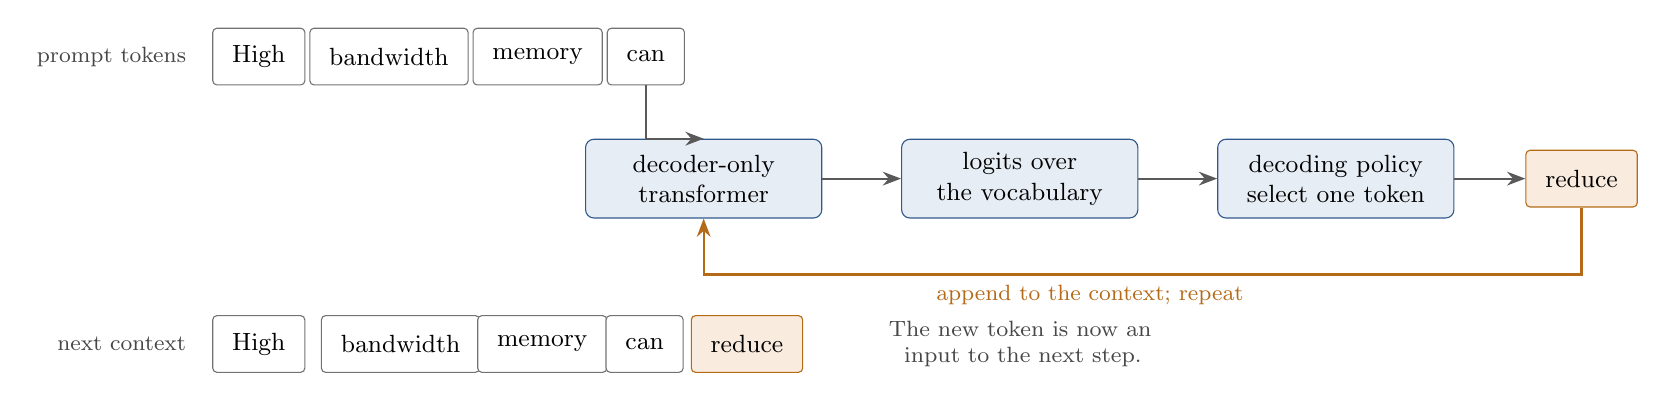
\begin{tikzpicture}[
  font=\small,
  ticket/.style={draw=black!55, fill=white, rounded corners=1.5pt,
                 minimum height=0.72cm, inner xsep=7pt, align=center},
  generated/.style={ticket, draw=hbmcol!85!black, fill=hbmcol!15},
  model/.style={draw=ddrcol!85!black, fill=ddrcol!12,
                rounded corners=3pt, minimum width=3.0cm,
                minimum height=1.0cm, align=center},
  flow/.style={-{Stealth}, thick, black!65},
  loop/.style={-{Stealth}, thick, hbmcol!85!black},
  note/.style={font=\footnotesize, text=black!72, align=center}
]
  \node[note, anchor=east] at (-6.35,1.2) {prompt tokens};
  \node[ticket] (p1) at (-5.55,1.2) {High};
  \node[ticket, right=0.05cm of p1] (p2) {bandwidth};
  \node[ticket, right=0.05cm of p2] (p3) {memory};
  \node[ticket, right=0.05cm of p3] (p4) {can};

  \node[model] (model) at (0.1,-0.35)
    {decoder-only\\transformer};
  \node[model, right=1.0cm of model] (logits)
    {logits over\\the vocabulary};
  \node[model, right=1.0cm of logits] (select)
    {decoding policy\\select one token};
  \node[generated, right=0.9cm of select] (new) {reduce};

  \draw[flow] (p4.south) |- (model.north);
  \draw[flow] (model) -- (logits);
  \draw[flow] (logits) -- (select);
  \draw[flow] (select) -- (new);
  \draw[loop] (new.south) -- ++(0,-0.85) -| (model.south)
    node[pos=0.28, below, note, text=hbmcol!85!black]
      {append to the context; repeat};

  \node[note, anchor=east] at (-6.35,-2.45) {next context};
  \node[ticket] at (-5.55,-2.45) {High};
  \node[ticket] at (-3.75,-2.45) {bandwidth};
  \node[ticket] at (-1.95,-2.45) {memory};
  \node[ticket] at (-0.65,-2.45) {can};
  \node[generated] at (0.65,-2.45) {reduce};
  \node[note, anchor=west, text width=4.9cm] at (1.55,-2.45)
    {The new token is now an input to the next step.};
\end{tikzpicture}%
}
\caption{Autoregressive generation at token level.  Token boundaries are
illustrative and depend on the tokenizer; the example is not intended to show
the output of a particular model.  Author's synthesis.}
\label{fig:token-generation}
\end{figure}

The \emph{context} at a given step comprises the prompt tokens and all tokens
generated so far.  Its maximum permitted length is the context window.  The
prompt length and requested generation length are separate workload
variables: the former controls how much history must initially be processed,
whereas the latter controls how many serial decode iterations are executed.
Batch size or concurrency determines how many sequences share an evaluation
step.  These quantities must not be collapsed into a model name when reporting
performance.

\subsection{What one model evaluation computes}

Most contemporary generative LLMs use a decoder-only transformer derived from
the attention architecture of Vaswani et al.~\cite{vaswani2017attention}.
Token identifiers are mapped to vectors, position information is incorporated,
and the vectors pass through a stack of transformer layers.  Each layer
contains causal self-attention, a feed-forward network and the associated
normalisation and residual operations.  The causal constraint prevents a
position from using later tokens.

For one attention head, learned projections form queries, keys and values,
\(Q=XW_Q\), \(K=XW_K\), and \(V=XW_V\).  A simplified attention operation is

\begin{equation}
\label{eq:scaled-dot-product-attention}
  \operatorname{Attention}(Q,K,V)
  = \operatorname{softmax}\!\left(
      \frac{QK^{\mathsf T}}{\sqrt{d_h}} + M_{\mathrm{causal}}
    \right)V,
\end{equation}
\eqcaption{Scaled dot-product causal attention.  The mask excludes future
positions; during decode, the new query uses keys and values retained from the
existing context.}

where \(d_h\) is the head dimension and \(M_{\mathrm{causal}}\) represents the
causal mask.  Multi-head attention performs several such projections, and the
feed-forward block applies large learned linear transformations independently
at each token position.  After the final layer, an output projection produces
the vocabulary logits used by the decoding policy.  Architectural variants
change details such as positional encoding, activation function, normalisation
and the number of key--value heads, but not the data-lifetime distinction used
in this thesis.

That distinction has three parts~\cite{pope2023efficient,sheng2023flexgen}:

\begin{itemize}
  \item \textbf{Weights} are the fixed learned parameters.  They persist for
        the model's lifetime, are reused by all requests and usually dominate
        its capacity footprint.
  \item The \textbf{key--value (KV) cache} retains the key and value vectors
        already computed in every layer.  It avoids recomputing the complete
        prefix at each decode step, but is private to a sequence, grows with
        context length and concurrency, and must be read when later tokens
        attend to their history.
  \item \textbf{Activations and workspaces} are temporary intermediates and
        runtime buffers.  Their sizes depend on the phase, batch, kernels and
        implementation; prepacked or duplicated weights may add another
        runtime-managed allocation.
\end{itemize}

The KV cache is therefore not the model's memory.  It is request state beside
the model, and the two objects have different lifetimes and access patterns.
PagedAttention demonstrates how variable-size KV allocations and
fragmentation can limit serving capacity even when the arithmetic is
unchanged~\cite{kwon2023pagedattention}.  That study targets GPU serving, so it
supports the memory-management mechanism rather than a quantitative claim
about the CPU studied here.

\subsection{The inference pipeline and its memory objects}

\figref{fig:inference-memory-lifetimes} follows one request through the
runtime.  Model loading and any weight repacking happen before steady-state
generation.  Tokenization produces the prompt identifiers.  \emph{Prefill}
processes those identifiers and creates the initial KV cache.  The
\emph{decode} loop then evaluates one new position per sequence, selects a
token and appends its key and value state.  Sampling and detokenization are
usually small compared with the transformer layers, but they are inside the
user-visible latency boundary unless the measurement deliberately excludes
them.

\begin{figure}[htbp]
\centering
\resizebox{\textwidth}{!}{%
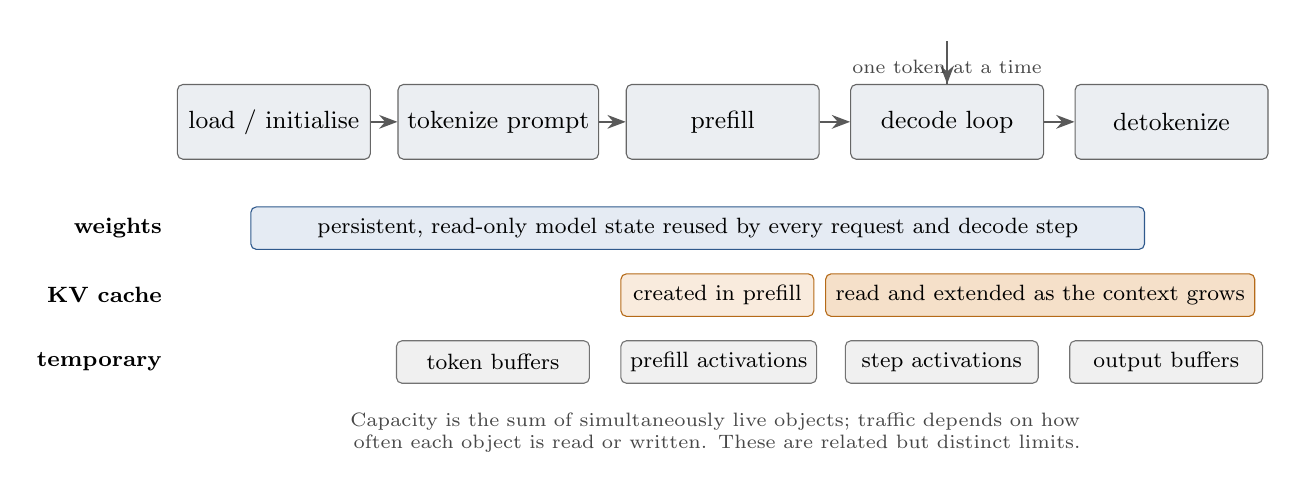
\begin{tikzpicture}[
  font=\small,
  stage/.style={draw=black!60, fill=neutralcol, rounded corners=2pt,
                minimum width=2.45cm, minimum height=0.95cm, align=center},
  flow/.style={-{Stealth}, thick, black!65},
  state/.style={rounded corners=2pt, minimum height=0.54cm, align=center,
                font=\footnotesize},
  label/.style={font=\footnotesize\bfseries, anchor=east},
  note/.style={font=\scriptsize, align=center, text=black!72}
]
  \node[stage] (load) at (-5.6,2.2) {load / initialise};
  \node[stage] (tok) at (-2.75,2.2) {tokenize prompt};
  \node[stage] (pre) at (0.1,2.2) {prefill};
  \node[stage] (dec) at (2.95,2.2) {decode loop};
  \node[stage] (out) at (5.8,2.2) {detokenize};
  \draw[flow] (load) -- (tok);
  \draw[flow] (tok) -- (pre);
  \draw[flow] (pre) -- (dec);
  \draw[flow] (dec) -- (out);
  \draw[flow] (dec.north) .. controls +(0,0.7) and +(0,0.7) .. (dec.north)
    node[above, note] {one token at a time};

  \node[label] at (-6.9,0.85) {weights};
  \node[state, draw=ddrcol!85!black, fill=ddrcol!13,
        minimum width=11.35cm, anchor=west] at (-5.9,0.85)
    {persistent, read-only model state reused by every request and decode step};

  \node[label] at (-6.9,0.0) {KV cache};
  \node[state, draw=hbmcol!85!black, fill=hbmcol!15,
        minimum width=2.45cm, anchor=west] (kvpre) at (-1.2,0.0)
    {created in prefill};
  \node[state, draw=hbmcol!85!black, fill=hbmcol!24,
        minimum width=5.45cm, anchor=west] at (1.4,0.0)
    {read and extended as the context grows};

  \node[label] at (-6.9,-0.85) {temporary};
  \node[state, draw=black!55, fill=black!6,
        minimum width=2.45cm, anchor=west] at (-4.05,-0.85)
    {token buffers};
  \node[state, draw=black!55, fill=black!6,
        minimum width=2.45cm, anchor=west] at (-1.2,-0.85)
    {prefill activations};
  \node[state, draw=black!55, fill=black!6,
        minimum width=2.45cm, anchor=west] at (1.65,-0.85)
    {step activations};
  \node[state, draw=black!55, fill=black!6,
        minimum width=2.45cm, anchor=west] at (4.5,-0.85)
    {output buffers};

  \node[note, text width=12.0cm] at (0,-1.75)
    {Capacity is the sum of simultaneously live objects; traffic depends on
     how often each object is read or written.  These are related but distinct
     limits.};
\end{tikzpicture}%
}
\caption{Inference stages and tensor lifetimes for one autoregressive
request.  The diagram separates persistent, growing and transient state; it
does not imply that every runtime materialises each buffer separately.
Author's synthesis, informed by Pope et al., FlexGen and
PagedAttention~\cite{pope2023efficient,sheng2023flexgen,kwon2023pagedattention}.}
\label{fig:inference-memory-lifetimes}
\end{figure}
\FloatBarrier

Three latency and throughput concepts follow directly.  \emph{Time to first
token} (TTFT) covers the request boundary through the first generated token and
is therefore driven largely, but not exclusively, by prefill.  \emph{Inter-token
latency} (ITL), also called time per output token, measures successive decode
steps.  Throughput in tokens per second depends on whether tokens are counted
for one sequence or across a batch.  These metrics answer different questions
and must be reported with prompt length, generated length and concurrency.

\subsection{Where memory can limit CPU inference}
\label{sec:inference-pipeline-bottlenecks}

The pipeline exposes several different memory problems; referring simply to
``the memory bottleneck'' hides the mechanism.  \tabref{tab:inference-pipeline}
separates them.  Na et al.'s CPU characterisation confirms that prefill and
decode stress the machine differently~\cite{na2024llmcpu}, while analytical
work across inference hardware explains the low arithmetic intensity of
small-batch generation~\cite{pope2023efficient,yuan2024roofline}.  Evidence
from accelerator serving is included where it identifies a tensor lifetime or
allocation problem, not as a prediction of a Xeon Max speedup.

\begin{table}[htbp]
\centering
\small
\tabsetup
\caption{Memory pressure along an LLM inference request.  ``Possible limit''
names a mechanism to test, not an assumption that it dominates every model or
runtime.}
\label{tab:inference-pipeline}
\begin{tabularx}{\textwidth}{@{}P{2.15cm}P{3.05cm}YP{3.0cm}@{}}
\toprule
\headrow
\textbf{Stage} & \textbf{Principal objects} & \textbf{Possible memory limit}
& \textbf{Treatment here} \\
\midrule
Load and initialise
& model file, weights, packed copies
& Storage I/O, page faults and temporary duplication determine startup and
  whether the resident model fits a tier.
& Measured separately; excluded from steady-state token rates. \\
\addlinespace[2pt]
Tokenize and prepare
& input text, token IDs, request metadata
& Usually small in bytes, but serial runtime work can enter TTFT.
& Kept inside end-to-end TTFT; not attributed to HBM without evidence. \\
\addlinespace[2pt]
Prefill
& weights, prompt activations, KV writes
& Long prompts expose matrix--matrix parallelism and temporary storage, while
  weights are reused across positions and the initial KV cache is written.
& Prompt-evaluation time and throughput reported separately. \\
\addlinespace[2pt]
Decode linear layers
& weights, small activations
& At low batch, little reuse is available before the next layer and the
  weight set may be streamed again for every token.
& Primary candidate for a bandwidth benefit; tested against Roofline and
  counters. \\
\addlinespace[2pt]
Decode attention
& growing KV cache, new key/value
& Dense attention reads an increasing history and appends new state; capacity
  grows with context and batch, and allocation can fragment.
& Context and concurrency sweep plus resident-set and placement checks. \\
\addlinespace[2pt]
Select and detokenize
& vocabulary scores, sampling and text buffers
& Small state but serial execution, synchronisation or runtime overhead can
  cap latency even when bandwidth is available.
& Included in user-visible latency; isolated before assigning causality. \\
\bottomrule
\end{tabularx}
\end{table}
\FloatBarrier

These limits interact.  Quantization shrinks the persistent weight stream but
does not necessarily shrink the KV cache; grouped-query or multi-query
attention reduces KV state; batching reuses weights but increases request
state; and long context increases KV traffic even when the weight footprint is
unchanged.  A working set may be \emph{capacity-bound} because it does not fit,
\emph{bandwidth-bound} because useful work waits for a sustained byte rate, or
\emph{latency/overhead-bound} because too few accesses are in flight to reach
that rate.  Only the second condition predicts a proportional benefit from a
faster memory tier.  \secref{sec:inference-model} develops the quantitative
tests for distinguishing these cases after the next two sections establish
the cluster and processor on which they occur.

\section{Model weights: representation, loading and use}
\label{sec:model-weights}

\subsection{Parameters and activations}

\textbf{Model weights} are learned numerical tensors: arrays with shapes
and element types that specify the model's transformations.  They
include embedding tables, attention projection matrices, feed-forward
matrices, learned normalization coefficients, and the output projection.
Some architectures tie the embedding and output tensors, so two uses need
not imply two independent allocations.  Ordinary inference uses the
trained parameters without updating them; no training gradients or
optimizer state are required for that computation.

A linear operation makes the distinction precise:
\begin{equation}
\label{eq:weights-activations}
 Y=XW,\qquad
 X\in\mathbb{R}^{m\times d_{\mathrm{in}}},\quad
 W\in\mathbb{R}^{d_{\mathrm{in}}\times d_{\mathrm{out}}},\quad
 Y\in\mathbb{R}^{m\times d_{\mathrm{out}}}.
\end{equation}
\eqcaption{A learned matrix \(W\) transforms \(m\) input activation
vectors into \(m\) new activation vectors.  Biases are omitted.}

Here \(W\) is persistent model data, whereas \(X\) and \(Y\) depend on
the positions being evaluated.  The same \(W\) can serve many positions
and many requests.  In attention, \(W_K\) and \(W_V\) are weights;
\(K=XW_K\) and \(V=XW_V\) are computed values.  Retaining these values
as KV state does not create additional trained parameters.  This
separation explains why the weight payload is principally a property of
the model and its representation, while KV payload also depends on the
workload's histories.

\subsection{From model files to runtime tensors}

A checkpoint or inference model file stores serialized tensors and
metadata describing such properties as names, shapes and numerical
representations.  Architecture configuration and tokenizer information
may be provided alongside it.  Large models can be split across several
files.  Files are persistent storage artifacts; kernels ultimately need
addressable tensor representations in the process's memory space.
\figref{fig:weight-loading} separates this preparation from repeated
execution.

One loading path reads tensor data and copies it into allocated buffers.
Another maps file-backed storage into the virtual address space.
\textbf{Memory mapping} establishes an addressable range without
necessarily populating all its physical pages immediately.  Accesses
can fault pages in on demand; prefetching and explicit population can
change when that cost occurs.  The runtime may use the mapped
representation directly or create additional tensors.  PyTorch's
checkpoint-loading documentation illustrates both mapped loading and
copying checkpoint tensors into a model's parameter allocations; these
are alternatives, not a universal loading sequence~\cite{pytorchloading2026}.

\begin{figure}[htbp]
\centering
% Vector schematic: preparation above, memory-to-cache-to-core traffic below.
% Icons are drawn locally so the figure stays scalable and matches the thesis.
\begingroup
\resizebox{\textwidth}{!}{%
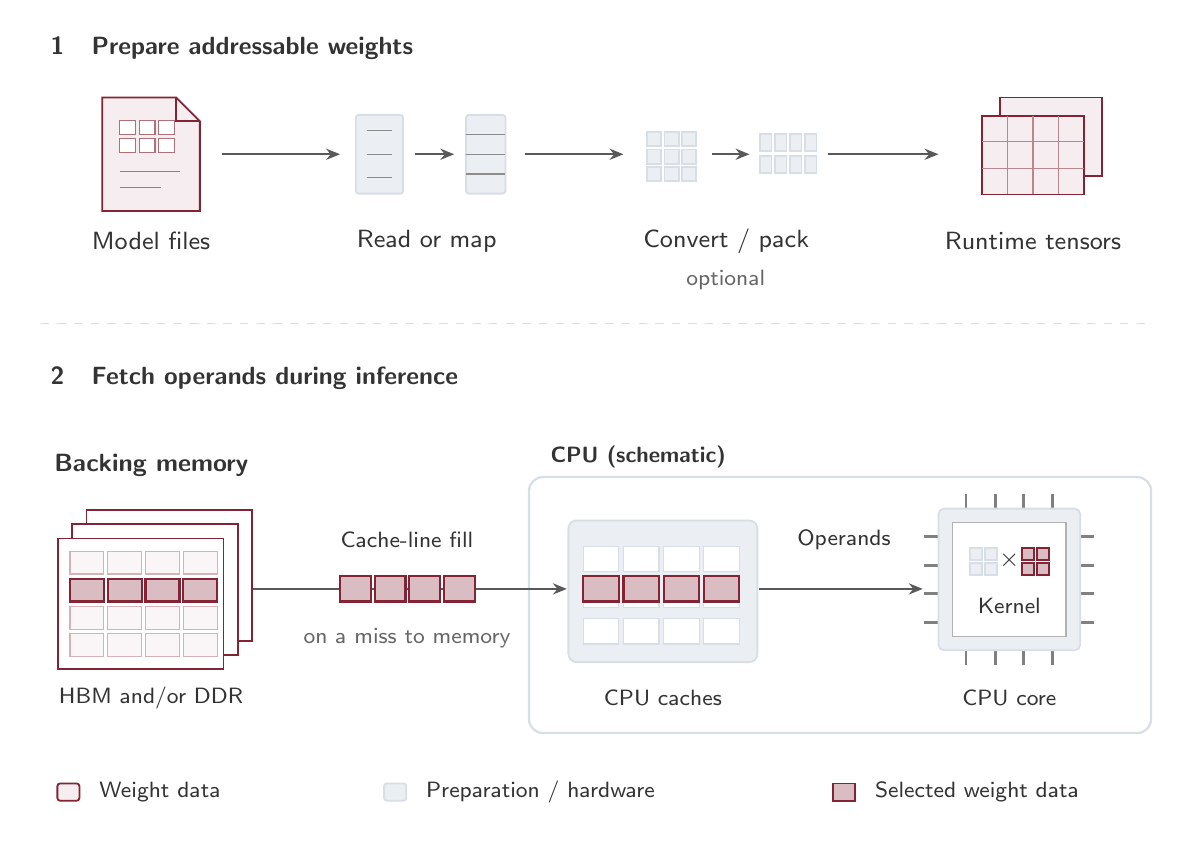
\begin{tikzpicture}[
 font=\small\sffamily,text=black!80,
 data/.style={draw=figcol,fill=figcol!8,line width=0.65pt},
 mechanism/.style={draw=tabline,fill=neutralcol,line width=0.65pt},
 flow/.style={-{Stealth[length=5pt,width=4pt]},draw=black!65,line width=0.85pt},
 note/.style={font=\footnotesize\sffamily,align=center},
 label/.style={align=center,text width=2.9cm},
 heading/.style={font=\small\sffamily\bfseries,anchor=west}
]
\node[heading] at (-0.9,1.6) {1\quad Prepare addressable weights};

% Serialized tensor file: a folded document with a numerical array and metadata.
\begin{scope}[shift={(0.5,0.25)}]
 \draw[data] (-0.62,-0.72)--(0.62,-0.72)--(0.62,0.42)
   --(0.32,0.72)--(-0.62,0.72)--cycle;
 \draw[draw=figcol,line width=0.65pt] (0.32,0.72)--(0.32,0.42)--(0.62,0.42);
 \foreach \x in {0,1,2} \foreach \y in {0,1}
  \draw[draw=figcol!65,fill=white] (-0.4+\x*0.25,0.02+\y*0.23)
   rectangle ++(0.2,0.18);
 \draw[draw=figcol!65] (-0.4,-0.22)--(0.37,-0.22);
 \draw[draw=figcol!65] (-0.4,-0.42)--(0.12,-0.42);
\end{scope}
\node[label] at (0.5,-0.85) {Model files};
\draw[flow] (1.4,0.25)--(2.9,0.25);

% Loading makes tensor bytes addressable: storage and memory buffer symbols.
\begin{scope}[shift={(4,0.25)}]
 \draw[mechanism,rounded corners=1pt] (-0.9,-0.5) rectangle (-0.3,0.5);
 \foreach \y in {-0.3,0,0.3}
  \draw[draw=black!45] (-0.76,\y)--(-0.44,\y);
 \draw[flow] (-0.15,0)--(0.35,0);
 \draw[mechanism,rounded corners=1pt] (0.5,-0.5) rectangle (1,0.5);
 \foreach \y in {-0.25,0,0.25}
  \draw[draw=black!45] (0.5,\y)--(1,\y);
\end{scope}
\node[label] at (4,-0.85) {Read or map};
\draw[flow] (5.25,0.25)--(6.5,0.25);

% Optional preparation: rearrange a matrix into a kernel-friendly layout.
\begin{scope}[shift={(7.8,0.25)}]
 \foreach \x in {0,1,2} \foreach \y in {0,1,2}
  \draw[mechanism] (-1+\x*0.22,-0.34+\y*0.22) rectangle ++(0.18,0.18);
 \draw[flow] (-0.18,0)--(0.3,0);
 \foreach \x in {0,1,2,3} \foreach \y in {0,1}
  \draw[mechanism] (0.43+\x*0.19,-0.24+\y*0.28) rectangle ++(0.15,0.22);
\end{scope}
\node[label] at (7.8,-0.85) {Convert / pack};
\node[note,text=black!60] at (7.8,-1.35) {optional};
\draw[flow] (9.1,0.25)--(10.5,0.25);

% Runtime representation: overlapping tensor planes, not physical page residency.
\begin{scope}[shift={(11.7,0.25)}]
 \draw[data] (-0.42,-0.28) rectangle (0.88,0.72);
 \draw[data] (-0.65,-0.51) rectangle (0.65,0.49);
 \foreach \x in {1,2,3}
  \draw[draw=figcol!55] (-0.65+\x*0.325,-0.51)--++(0,1);
 \foreach \y in {1,2}
  \draw[draw=figcol!55] (-0.65,-0.51+\y/3)--++(1.3,0);
\end{scope}
\node[label] at (11.7,-0.85) {Runtime tensors};
\draw[draw=tabline,dashed] (-0.9,-1.9)--(13.2,-1.9);

\node[heading] at (-0.9,-2.6) {2\quad Fetch operands during inference};

% Main-memory pages: one contiguous row is selected for the illustrated fill.
\node[label,font=\small\sffamily\bfseries] at (0.5,-3.7) {Backing memory};
\begin{scope}[shift={(0.5,-5.15)}]
 \draw[data,fill=white] (-0.82,-0.78) rectangle (1.28,0.88);
 \draw[data,fill=white] (-1.0,-0.96) rectangle (1.1,0.7);
 \draw[data,fill=white] (-1.18,-1.14) rectangle (0.92,0.52);
 \foreach \x in {0,1,2,3} \foreach \y in {0,1,2,3}
  \draw[draw=figcol!35,fill=figcol!4]
   (-1.03+\x*0.48,-0.98+\y*0.35) rectangle ++(0.43,0.29);
 \foreach \x in {0,1,2,3}
  \draw[data,fill=figcol!30,line width=0.8pt]
   (-1.03+\x*0.48,-0.28) rectangle ++(0.43,0.29);
\end{scope}
\node[note] at (0.5,-6.65) {HBM and/or DDR};

% CPU boundary contains the cache hierarchy and the executing core.
\draw[draw=tabline,rounded corners=5pt,line width=0.8pt]
 (5.3,-3.85) rectangle (13.2,-7.1);
\node[note,anchor=west,font=\footnotesize\sffamily\bfseries]
 at (5.45,-3.6) {CPU (schematic)};

% Cache rows show retained copies; highlight only the illustrated line.
\begin{scope}[shift={(7,-5.15)}]
 \draw[mechanism,rounded corners=3pt] (-1.2,-1.05) rectangle (1.2,0.75);
 \foreach \x in {0,1,2,3} \foreach \y in {0,1,2}
  \draw[draw=tabline,fill=white]
   (-1.01+\x*0.51,-0.82+\y*0.46) rectangle ++(0.45,0.32);
 \foreach \x in {0,1,2,3}
  \draw[data,fill=figcol!30,line width=0.8pt]
   (-1.01+\x*0.51,-0.28) rectangle ++(0.45,0.32);
\end{scope}
\node[note] at (7,-6.65) {CPU caches};

% A cache-line packet on the data path makes the transfer granularity visible.
\draw[flow] (1.8,-5.27)--(5.78,-5.27);
\foreach \x in {0,1,2,3}
 \draw[data,fill=figcol!30,line width=0.8pt]
  (2.9+\x*0.44,-5.43) rectangle ++(0.39,0.32);
\node[note] at (3.75,-4.65) {Cache-line fill};
\node[note,text=black!60] at (3.75,-5.9) {on a miss to memory};

% Core package with pins and a small matrix multiplication kernel.
\begin{scope}[shift={(11.4,-5.15)}]
 \foreach \p in {-0.55,-0.18,0.18,0.55} {
  \draw[draw=black!50,line width=1pt] (\p,-0.9)--(\p,-1.08);
  \draw[draw=black!50,line width=1pt] (\p,0.9)--(\p,1.08);
  \draw[draw=black!50,line width=1pt] (-0.9,\p)--(-1.08,\p);
  \draw[draw=black!50,line width=1pt] (0.9,\p)--(1.08,\p);
 }
 \draw[mechanism,rounded corners=2pt] (-0.9,-0.9) rectangle (0.9,0.9);
 \draw[draw=black!30,fill=white] (-0.72,-0.72) rectangle (0.72,0.72);
 \foreach \x in {0,1} \foreach \y in {0,1} {
  \draw[mechanism] (-0.5+\x*0.19,0.06+\y*0.19) rectangle ++(0.15,0.15);
  \draw[data,fill=figcol!30] (0.16+\x*0.19,0.06+\y*0.19) rectangle ++(0.15,0.15);
 }
 \node[font=\small\sffamily] at (0,0.24) {$\times$};
 \node[note] at (0,-0.34) {Kernel};
\end{scope}
\node[note] at (11.4,-6.65) {CPU core};
\draw[flow] (8.22,-5.27)--(10.3,-5.27);
\node[note] at (9.3,-4.65) {Operands};

% Legend uses swatches, with an additional key for the highlighted data line.
\node[data,rounded corners=1pt,minimum width=0.28cm,
 minimum height=0.22cm,inner sep=0pt] at (-0.55,-7.85) {};
\node[note,anchor=west] at (-0.28,-7.85) {Weight data};
\node[mechanism,rounded corners=1pt,minimum width=0.28cm,
 minimum height=0.22cm,inner sep=0pt] at (3.6,-7.85) {};
\node[note,anchor=west] at (3.87,-7.85) {Preparation / hardware};
\node[data,fill=figcol!30,minimum width=0.28cm,
 minimum height=0.22cm,inner sep=0pt] at (9.3,-7.85) {};
\node[note,anchor=west] at (9.57,-7.85) {Selected weight data};
\end{tikzpicture}%
}
\endgroup

\caption{From model files to weight operands.  The upper path shows
preparation of addressable tensors: reading and mapping are alternatives,
and conversion or packing is optional.  Mapping does not imply immediate
physical residency.  Below, a highlighted row illustrates weight data
fetched from backing memory into CPU caches as a cache-line fill; a
kernel then uses its operands.  Cache hits reuse retained data without
another main-memory transfer.  Pages can become resident during startup
or on demand.  Array cells and hardware drawings are schematic; the cache
hierarchy and transfers within it are collapsed.}
\label{fig:weight-loading}
\end{figure}
\FloatBarrier

Representation preparation can convert element types, unpack or pack
quantized blocks, or arrange matrices in a layout suited to a kernel.
\textbf{Packing} changes the storage order or layout to make accesses
and arithmetic more efficient; it need not change the represented
values or their precision.  Such preparation can use temporary buffers
or retain an additional representation.  A loader's peak memory use can
therefore exceed the final tensor payload.  A short loading timer also
does not prove that every mapped page has already been read from storage.

The operating system backs virtual addresses with physical pages.
Where these pages reside depends on the allocation type, page-fault
behavior and applicable memory policy, as well as on the loading path.
File-backed mappings and anonymous tensor allocations need not obey the
same locality assumptions.  In particular, the thread that prepares a
representation and the threads that later read it may run on different
CPU locality domains.  Allocation locality is developed in
\secref{sec:cpu-memory-systems}.

\subsection{Repeated use and numerical representation}

Once prepared, weights can remain available across requests.  This
avoids repeating file loading, but it does not keep all weights
permanently in CPU caches.  Each kernel requests its operands through
the cache hierarchy; cache misses fetch data from the backing memory.
A large weight working set can require repeated main-memory traffic
across layer evaluations and generation steps.  Model loading is thus
a storage-to-memory preparation activity, whereas operand fetching is
part of ongoing computation.

Access behavior also depends on the operation.  A dense matrix product
uses its matrix entries across the evaluated activation rows.  An
embedding lookup selects rows for particular token IDs and does not
necessarily read the whole embedding table.  Sparse or conditionally
activated architectures can use subsets of their parameters.  It is
therefore unsafe to equate the full model size with the exact bytes read
on every generation step.

FP32 stores four bytes per scalar; FP16 and BF16 store two, with
different distributions of exponent and significand bits.  Quantization
represents values with fewer bits and uses associated information, such
as scale factors and sometimes zero points, to interpret groups of
values.  A nominal four-bit weight payload is half a byte per parameter,
but its format also stores metadata and may add padding.  Not all
tensors must use the same type.  Kernels may compute directly on a
compressed representation or reconstruct values as part of execution;
the accumulation type can differ from the stored type.  Storage savings
therefore do not by themselves establish either arithmetic speed or
numerical quality~\cite{llamacppproject2026}.

A parameter count describes how many learned scalar values a model has,
not its file size, process memory footprint, or inference traffic.  The
next sections identify the other data retained by inference, before
\secref{sec:memory-requirements} combines their capacity estimates.
\FloatBarrier

\section{Autoregressive inference and KV state}
\label{sec:autoregressive-kv}

\subsection{Prefill and decode}

Autoregressive generation selects a new token from the model's
next-token distribution and extends the prefix before producing another:
\begin{equation}
\label{eq:autoregressive-factorization}
 p(x_1,\ldots,x_T)=\prod_{t=1}^{T}p(x_t\mid x_{<t}).
\end{equation}
\eqcaption{Autoregressive factorization: each token is conditioned on
the preceding tokens.}

The model's logits can be turned into probabilities and a token can be
selected deterministically or by sampling.  Generation stops at a
termination token or another declared limit.  These choices affect the
output, but the important execution dependency is that a sequence's
next token must be known before its following evaluation can proceed.
Different sequences can nevertheless advance together.

\textbf{Prefill} evaluates the prompt.  Its positions can be processed
in parallel within matrix operations because the token IDs are already
known, while the causal mask prevents attention to future positions.
For ordinary generation, the logits at the last prompt position produce
the first output token.  \textbf{Decode} then evaluates newly generated
tokens, conventionally one new position per active sequence per step.
Evaluating that first output token produces the distribution for the
second output token.  Thus producing \(O\) output tokens normally needs
prefill and \(O-1\) subsequent decode evaluations; the final emitted
token need not itself be evaluated unless further generation is needed.
Chunked prompt processing and other execution strategies can change how
these logical phases are scheduled, without changing this dependency.

\subsection{What the cache retains}

At each layer, the input activations generate keys and values using the
layer's trained projections.  A later position's query compares against
the available keys, and the resulting attention coefficients combine
the associated values.  Since earlier positions cannot attend to later
ones under causal attention, their keys and values need not be recomputed
when the sequence is extended.  The \textbf{KV cache} retains these
per-layer values for reuse~\cite{pope2023efficient}.

Prefill establishes entries for the evaluated prompt positions.  Decode
reads the retained history and adds entries for the position being
processed.  Queries and most intermediate activations are temporary;
keys and values persist for as long as the corresponding history is
needed.  The cache avoids repeating computation of the previous
positions' KV state; it does not eliminate reading that state or
computing attention for a new query.  With full-history attention, longer
histories increase both retained payload and the state a query can access.
The logical attention expression need not be implemented by materializing
its whole score matrix; kernels can operate on tiles.

The number of \textbf{KV heads} controls how many distinct key/value
vectors are retained per position.  In multi-head attention (MHA), each
query head has its own KV head.  Multi-query attention (MQA) shares one
KV head across all query heads.  Grouped-query attention (GQA) shares a
KV head within each group of query heads, giving an intermediate KV
count~\cite{ainslie2023gqa}.  For fixed layer count, head dimension,
precision and retained length, fewer KV heads reduce the KV payload
proportionally.  The query-head count can remain larger, so a small KV
payload does not mean that all attention computation shrinks by the same
factor.  The attention arrangement is a property of the model architecture,
not a storage policy chosen freely by an allocator.

\subsection{Logical history and physical storage}

A sequence has a logical set of valid KV entries.  A runtime may store
these in a contiguous buffer or map them to fixed-size physical blocks.
Block allocation accommodates sequences of different lengths without
requiring one contiguous maximum-length buffer for each
sequence~\cite{kwon2023pagedattention}.  The PagedAttention work develops
this mechanism for GPU serving; its distinction between logical tokens
and physical blocks is also useful when describing CPU runtime storage,
without assuming identical implementation or performance.

Four quantities must remain distinct.  \textbf{Populated entries} hold
valid state for evaluated positions.  \textbf{Occupied blocks} include
storage assigned to these entries and any unused space within their
blocks.  \textbf{Reserved pool capacity} is the storage set aside for
KV management, including blocks not currently assigned to requests.
\textbf{Resident memory} is the portion currently backed by physical
pages in RAM.  A reserved virtual allocation, a committed pool and its
resident pages can have different sizes.  Lazy page population, eager
initialization and operating-system behavior affect their relationship.

For example, with 16 positions per block, a 17-position sequence occupies
two blocks: 32 positions of block capacity but only 17 populated entries.
A pool of 100 such blocks reserves 1{,}600 positions of capacity even if
only those two blocks are occupied.  Completing the request releases its
logical ownership, but a runtime can keep the pool allocated for later
requests.  Process memory need not drop when the request finishes.
\figref{fig:inference-memory-lifetimes} shows these distinct lifetimes.

\begin{figure}[htbp]
\centering
% Storyboard: one request, shared weights, KV slots inside a reusable pool.
% Filled cells represent valid state; clearing ownership need not erase bytes.
\begingroup
\resizebox{\textwidth}{!}{%
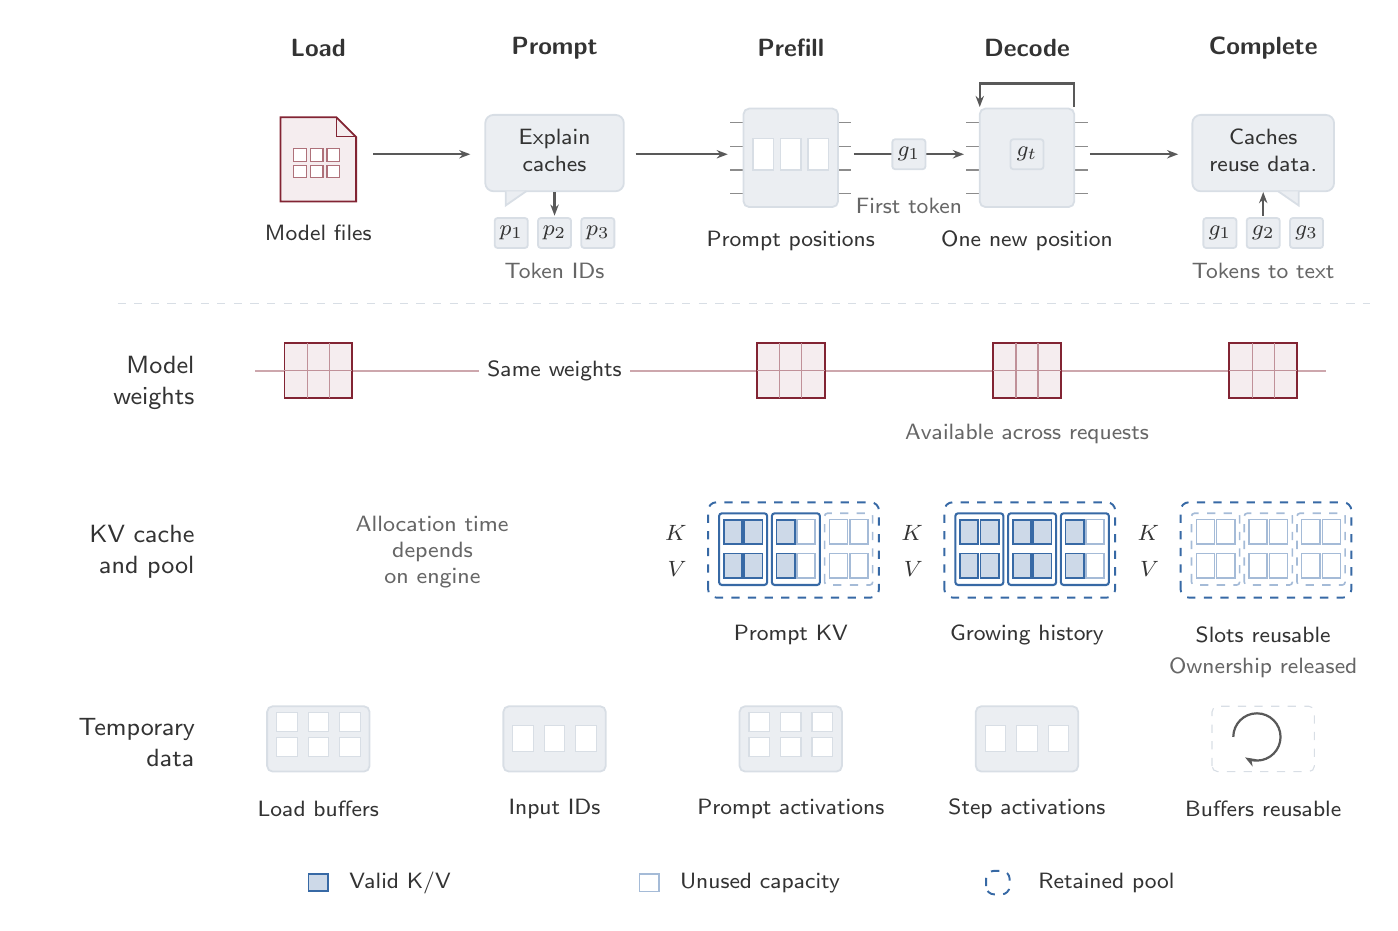
\begin{tikzpicture}[
 font=\small\sffamily,text=black!80,
 weight/.style={draw=figcol,fill=figcol!8,line width=0.65pt},
 temp/.style={draw=tabline,fill=neutralcol,line width=0.65pt},
 kv/.style={draw=ddrcol,fill=ddrcol!25,line width=0.65pt},
 free/.style={draw=ddrcol!45,fill=white,line width=0.5pt},
 flow/.style={-{Stealth[length=4pt,width=3pt]},draw=black!65,line width=0.8pt},
 note/.style={font=\footnotesize\sffamily,align=center},
 stage/.style={font=\small\sffamily\bfseries,align=center},
 rowlabel/.style={anchor=east,align=right,text width=2.0cm},
 token/.style={temp,rounded corners=1pt,minimum width=0.42cm,
   minimum height=0.38cm,inner sep=1pt,font=\footnotesize\sffamily},
 pool/.style={draw=ddrcol,dashed,rounded corners=3pt,line width=0.7pt}
]

% The request path: files, prompt, parallel prompt work, serial steps, text.
\node[stage] at (0,1.7) {Load};
\node[stage] at (3,1.7) {Prompt};
\node[stage] at (6,1.7) {Prefill};
\node[stage] at (9,1.7) {Decode};
\node[stage] at (12,1.7) {Complete};

% Document icon used for model loading.
\draw[weight] (-0.48,-0.25)--(0.48,-0.25)--(0.48,0.57)
 --(0.23,0.82)--(-0.48,0.82)--cycle;
\draw[draw=figcol] (0.23,0.82)--(0.23,0.57)--(0.48,0.57);
\foreach \x in {0,1,2} \foreach \y in {0,1}
 \draw[draw=figcol!65,fill=white]
  (-0.31+\x*0.21,0.05+\y*0.21) rectangle ++(0.16,0.16);
\node[note] at (0,-0.65) {Model files};

% Text enters as a prompt; token identifiers are shown below it.
\draw[temp,rounded corners=3pt] (2.12,-0.12) rectangle (3.88,0.85);
\draw[temp] (2.38,-0.12)--(2.38,-0.3)--(2.64,-0.12);
\node[note] at (3,0.4) {Explain\\caches};
\foreach \j/\dx in {1/-0.55,2/0,3/0.55}
 \node[token] at (3+\dx,-0.65) {$p_{\j}$};
\draw[flow] (3,-0.13)--(3,-0.43);
\node[note,text=black!60] at (3,-1.13) {Token IDs};

% Small processor icons: several known prompt positions, then one new position.
\foreach \cx in {6,9} {
 \foreach \dy in {-0.15,0.15,0.45,0.75} {
  \draw[draw=black!45] (\cx-0.6,\dy)--(\cx-0.77,\dy);
  \draw[draw=black!45] (\cx+0.6,\dy)--(\cx+0.77,\dy);
 }
 \draw[temp,rounded corners=2pt] (\cx-0.6,-0.32) rectangle (\cx+0.6,0.93);
}
\foreach \dx in {-0.35,0,0.35}
 \draw[temp,fill=white] (6+\dx-0.13,0.15) rectangle ++(0.26,0.4);
\node[token] at (9,0.35) {$g_t$};
\node[note] at (6,-0.75) {Prompt positions};
\node[note] at (9,-0.75) {One new position};
\draw[flow] (9.6,0.95)--(9.6,1.25)--(8.4,1.25)--(8.4,0.95);

% Emission follows prefill as well as decode; the loop evaluates emitted tokens.
\draw[flow] (0.7,0.35)--(1.93,0.35);
\draw[flow] (4.03,0.35)--(5.2,0.35);
\draw[flow] (6.8,0.35)--(8.2,0.35);
\node[token] at (7.5,0.35) {$g_1$};
\node[note,text=black!60] at (7.5,-0.3) {First token};
\draw[flow] (9.8,0.35)--(10.92,0.35);
\draw[temp,rounded corners=3pt] (11.1,-0.12) rectangle (12.9,0.85);
\draw[temp] (12.45,-0.12)--(12.45,-0.3)--(12.19,-0.12);
\node[note] at (12,0.4) {Caches\\reuse data.};
\foreach \j/\dx in {1/-0.55,2/0,3/0.55}
 \node[token] at (12+\dx,-0.65) {$g_{\j}$};
\draw[flow] (12,-0.43)--(12,-0.13);
\node[note,text=black!60] at (12,-1.13) {Tokens to text};

\draw[draw=tabline,dashed] (-2.55,-1.55)--(13.35,-1.55);

% The same trained matrices remain available for the engine's lifetime.
\node[rowlabel] at (-1.45,-2.55) {Model\\weights};
\draw[draw=figcol!40,line width=0.7pt] (-0.8,-2.4)--(12.8,-2.4);
\foreach \cx in {0,6,9,12} {
 \draw[weight] (\cx-0.43,-2.75) rectangle (\cx+0.43,-2.05);
 \foreach \dx in {-0.14,0.14}
  \draw[draw=figcol!50] (\cx+\dx,-2.75)--(\cx+\dx,-2.05);
 \draw[draw=figcol!50] (\cx-0.43,-2.4)--(\cx+0.43,-2.4);
}
\node[note,fill=white,inner sep=3pt] at (3,-2.4) {Same weights};
\node[note,text=black!60] at (9,-3.2) {Available across requests};

% Three snapshots of one fixed-capacity pool, each with three two-position blocks.
% A slot comprises the K and V cells in one column; widths are illustrative.
\node[rowlabel] at (-1.45,-4.7) {KV cache\\and pool};
\node[note,text width=2.1cm,text=black!60] at (1.45,-4.7)
 {Allocation time\\depends on engine};
\foreach \cx/\used in {6/3,9/5,12/0} {
 \draw[pool] (\cx-1.05,-5.28) rectangle (\cx+1.12,-4.07);
 \node[note,anchor=east] at (\cx-1.2,-4.46) {$K$};
 \node[note,anchor=east] at (\cx-1.2,-4.91) {$V$};
 \foreach \block in {0,1,2} {
  \pgfmathtruncatemacro{\blockstart}{2*\block}
  \ifnum\blockstart<\used
   \draw[draw=ddrcol,line width=0.75pt,rounded corners=1pt]
    (\cx-0.91+\block*0.67,-5.12) rectangle ++(0.61,0.91);
  \else
   \draw[draw=ddrcol!45,dashed,line width=0.6pt,rounded corners=1pt]
    (\cx-0.91+\block*0.67,-5.12) rectangle ++(0.61,0.91);
  \fi
  \foreach \slot in {0,1} {
   \pgfmathtruncatemacro{\entry}{2*\block+\slot}
   \foreach \dy in {-4.6,-5.03} {
    \ifnum\entry<\used
     \draw[kv] (\cx-0.85+\block*0.67+\slot*0.26,\dy)
      rectangle ++(0.23,0.31);
    \else
     \draw[free] (\cx-0.85+\block*0.67+\slot*0.26,\dy)
      rectangle ++(0.23,0.31);
    \fi
   }
  }
 }
}
\node[note] at (6,-5.75) {Prompt KV};
\node[note] at (9,-5.75) {Growing history};
\node[note] at (12,-5.75) {Slots reusable};
\node[note,text=black!60] at (12,-6.18) {Ownership released};

% Stage-local data: compact input buffers, activation arrays and reusable buffers.
\node[rowlabel] at (-1.45,-7.12) {Temporary\\data};
\foreach \cx in {0,3,6,9} {
 \draw[temp,rounded corners=2pt] (\cx-0.65,-7.49) rectangle (\cx+0.65,-6.66);
}
\foreach \cx in {0,6} \foreach \dx in {-0.4,0,0.4} \foreach \dy in {-7.3,-6.98}
 \draw[draw=tabline,fill=white] (\cx+\dx-0.13,\dy) rectangle ++(0.26,0.24);
\foreach \dx in {-0.4,0,0.4} {
 \draw[draw=tabline,fill=white] (3+\dx-0.13,-7.23) rectangle ++(0.26,0.32);
 \draw[draw=tabline,fill=white] (9+\dx-0.13,-7.23) rectangle ++(0.26,0.32);
}
\draw[draw=tabline,dashed,rounded corners=2pt]
 (11.35,-7.49) rectangle (12.65,-6.66);
\draw[flow] (11.62,-7.05) arc[start angle=180,end angle=-120,radius=0.3cm];
\node[note] at (0,-7.96) {Load buffers};
\node[note] at (3,-7.96) {Input IDs};
\node[note] at (6,-7.96) {Prompt activations};
\node[note] at (9,-7.96) {Step activations};
\node[note] at (12,-7.96) {Buffers reusable};

% Keys distinguish populated KV data from capacity without colour-name labels.
\node[kv,minimum width=0.25cm,minimum height=0.22cm,inner sep=0pt]
 at (0,-8.9) {};
\node[note,anchor=west] at (0.27,-8.9) {Valid K/V};
\node[free,minimum width=0.25cm,minimum height=0.22cm,inner sep=0pt]
 at (4.2,-8.9) {};
\node[note,anchor=west] at (4.47,-8.9) {Unused capacity};
\draw[pool] (8.48,-9.05) rectangle (8.78,-8.75);
\node[note,anchor=west] at (9.02,-8.9) {Retained pool};
\end{tikzpicture}%
}
\endgroup

\caption{Request stages and reusable storage in a persistent engine.
Prefill evaluates prompt tokens \(p_i\) and emits \(g_1\); decode
evaluates generated tokens sequentially.  KV state grows from three to
five evaluated positions within a six-position pool.  Paired K/V cells
hold valid entries; solid block outlines mark assigned blocks.
Completing this unshared request releases its slots while the pool can
remain allocated.  Empty cells indicate unused capacity, not erased
bytes.  Weights persist; temporary buffers may be reused.  Token examples
and dimensions are schematic, and pool allocation time and physical
residency depend on the runtime and memory policy.  The final emitted
token need not have a KV entry.}
\label{fig:inference-memory-lifetimes}
\end{figure}
\FloatBarrier

Sequences are not always physically independent.  \textbf{Prefix caching}
can reuse compatible KV blocks for a common prefix; reference counting
allows several requests to share these blocks.  Compatibility depends
on the model and the context that produced the state, not merely on
matching a suffix of text.  Shared blocks must remain valid while in
use, and an engine may keep reusable prefix blocks after individual
requests complete~\cite{vllmprefix2026}.  Summing every sequence's logical
length therefore gives an unshared payload estimate, not necessarily
the number of physical bytes occupied.  Sliding-window or other bounded
attention arrangements can also limit retained history.  Capacity models
must state which attention and sharing assumptions they use.
\FloatBarrier

\section{Inference engines and CPU execution}
\label{sec:inference-engines}

An \textbf{inference engine} connects a model's mathematical operations
to executable kernels and manages the data and requests surrounding
those operations.  It loads model representations, prepares inputs,
allocates KV storage and workspaces, dispatches numerical kernels, and
returns generated tokens.  Serving engines additionally manage queues,
request admission and scheduling.  These responsibilities determine when
computation happens and which allocations coexist, even when two
engines evaluate the same model.

\lcpp{} and vLLM are examples with different interfaces, representation
support and execution paths~\cite{llamacppproject2026,vllm2026}.  Their
names do not uniquely specify a kernel or memory policy: backend,
build options, model format and version all matter.  The background uses
engines to illustrate responsibilities; the experimental chapters must
identify the actual implementations and configurations compared.

\subsection{Requests, sequences and execution batches}

\textbf{Concurrency} counts requests or sequences active within a
stated observation boundary.  An \textbf{execution batch} is the set of
positions submitted together in one model evaluation.  A decode batch
can contain one position from each selected sequence, whereas a prefill
batch can contain many positions from one or several prompts.  Queueing,
chunking and admission limits can leave some concurrent requests outside
a particular execution batch.  Request count, sequence count and number
of evaluated positions should therefore be named separately.

For instance, 32 requests can be active while an engine evaluates only
eight sequences in a decode batch.  Alternatively, one prompt can supply
hundreds of positions to a prefill evaluation.  Continuous batching
allows completed sequences to leave and new work to enter between
iterations, changing both the amount of numerical work and the KV
histories being accessed~\cite{kwon2023pagedattention}.  An execution batch
can increase weight reuse, but its effect on response latency depends
also on waiting and scheduling.

\subsection{Kernels, parallelism and precision}

A \textbf{kernel} implements a numerical operation such as a matrix
product, normalization, embedding lookup or attention.  Dense products
with several activation rows can use matrix-matrix operations; a
single activation row gives a matrix-vector-like case.  Optimized
implementations tile work so that subsets of operands can be reused in
caches or registers.  Fusing operations can reduce intermediate writes,
but may change workspace needs and parallelization opportunities.

CPU execution combines instruction-level parallelism with work shared
across cores.  SIMD instructions process several values per instruction;
some processors provide matrix instructions for supported types.
Threads can divide output elements, matrix tiles or attention work.
Their efficiency depends on sufficient independent work, synchronization
cost, load balance and the locality of their operands.  Adding threads
can improve utilization until a compute resource or memory path
saturates; it can also introduce overhead or remote accesses.  Logical
hardware threads are not equivalent to additional physical cores.

The types used for weights, KV storage, temporary activations and
accumulation need not match.  Quantized weights can coexist with BF16
activations and a different KV type.  Lower storage precision changes
the capacity and traffic models, while the supported instructions and
conversion costs determine its execution consequences.  Numerical
accuracy and generated outputs must be evaluated under the chosen
representation rather than assumed identical after quantization.

For performance analysis, phase timers should be complemented by an
understanding of the dispatched kernels and runtime work.  Tokenization,
sampling, scheduling, allocation and synchronization contribute time
without necessarily appearing in a matrix kernel's operation count.
The distinction becomes particularly relevant for small batches or
short requests, where fixed overhead is a larger fraction of elapsed
time~\cite{na2024llmcpu}.

\section{CPU memory systems}
\label{sec:cpu-memory-systems}

\subsection{Caches, main memory and physical residency}

A CPU load or store uses a virtual address that is translated to a
physical page.  Data is transferred through a hierarchy of registers,
CPU caches and main memory.  Caches retain recently used cache lines,
not whole model objects as an indivisible unit.  A cache hit can serve
an access without fetching the line from main memory; a miss requires
data from a lower level.  Cache levels differ in capacity, latency and
sharing, and the exact organization is processor dependent.

The \textbf{working set} is the data used during the interval under
study.  Cache capacity can allow a tile of a large matrix to be reused
even when the complete model is much larger than the last-level cache.
Conversely, a tensor's presence in RAM does not imply a cache hit.
Stores also generate traffic: modified cache lines eventually need
writeback, and some store paths fetch a line before updating it.  The
bytes logically consumed by a kernel are consequently different from
the bytes observed at a memory controller.

File size describes persistent storage.  Virtual address space describes
addressable ranges.  Allocated capacity describes storage assigned to
objects or pools.  \textbf{Physical residency} describes which pages are
currently backed in RAM.  Operating-system resident-set measurements
must be interpreted with care when pages are shared or file backed;
summing process footprints can count shared pages more than once.
These quantities answer different questions and should not be used as
interchangeable measures of model memory use.

\subsection{HBM, DDR and memory modes}

\textbf{DDR} is conventional system DRAM accessed through memory
channels.  \textbf{HBM} uses stacked DRAM and a wide interface to provide
high aggregate bandwidth.  In CPU systems combining them, HBM generally
offers a smaller high-bandwidth resource and DDR a larger capacity
resource; usable sizes and attainable rates depend on the platform.
HBM's bandwidth advantage does not establish a lower latency for every
access pattern~\cite{intelmaxoverview,ibeid2025aurora}.

\textbf{Bandwidth} is transferred bytes per unit time,
\textbf{latency} is the time to complete an access, and
\textbf{capacity} is the amount held at once.  Concurrent independent
misses can hide part of the latency and sustain bandwidth.  A dependent
load chain can remain latency limited even when measured bandwidth is
low.  A working set can fit in a tier yet fail to use its bandwidth, or
require more capacity than that tier provides despite modest traffic.

In a separately addressable, often called \textbf{Flat}, configuration,
software can allocate physical pages from exposed memory domains.
Placement can then determine which tier backs weight tensors or KV
storage.  In a hardware-managed \textbf{Cache} configuration, HBM acts
as a cache for DDR backing memory; software does not assign every tensor
a separate HBM address range in the same way~\cite{intelmaxoverview}.
\figref{fig:cpu-memory-organization} shows the distinction.  Neither
mode is a universal default; the actual firmware mode and exposed
memory topology belong to the platform description.

\begin{figure}[htbp]
\centering
% Flat and Cache mode only; allocation choices and access paths are distinct.
\begingroup
\newcommand{\modecore}[1]{%
 \begin{scope}[shift={(#1,0.65)}]
  \foreach \p in {-0.4,0,0.4} {
   \draw[draw=black!45] (\p,-0.55)--(\p,-0.7);
   \draw[draw=black!45] (\p,0.55)--(\p,0.7);
   \draw[draw=black!45] (-0.65,\p)--(-0.8,\p);
   \draw[draw=black!45] (0.65,\p)--(0.8,\p);
  }
  \draw[hardware,rounded corners=2pt] (-0.65,-0.55) rectangle (0.65,0.55);
  \foreach \x in {-0.4,0.05} \foreach \y in {-0.32,0.1}
   \draw[draw=tabline,fill=white] (\x,\y) rectangle ++(0.35,0.24);
 \end{scope}
 \node[note,anchor=west] at (#1+1.0,0.65) {Cores};
 \begin{scope}[shift={(#1,-0.95)}]
  \draw[hardware,rounded corners=2pt] (-0.9,-0.4) rectangle (0.9,0.4);
  \foreach \x in {-0.68,-0.23,0.22} \foreach \y in {-0.25,0.08}
   \draw[draw=tabline,fill=white] (\x,\y) rectangle ++(0.37,0.2);
 \end{scope}
 \node[note,anchor=west] at (#1+1.08,-0.95) {CPU caches};
 \draw[access] (#1,-0.09)--(#1,-0.53);
}
\newcommand{\modestack}[2]{%
 \begin{scope}[shift={(#1,#2)}]
  \foreach \dy in {0,0.22,0.44}
   \draw[draw=hbmcol,fill=hbmcol!12,line width=0.65pt]
    (-0.8,\dy)--(0.45,\dy)--(0.9,\dy+0.35)
    --(-0.35,\dy+0.35)--cycle;
  \foreach \dx in {-0.25,0.15,0.55}
   \draw[draw=hbmcol!60] (\dx,0.46)--++(0.24,0.18);
 \end{scope}
}
\newcommand{\modedimm}[2]{%
 \begin{scope}[shift={(#1,#2)}]
  \draw[draw=ddrcol,fill=ddrcol!8,rounded corners=1pt,line width=0.65pt]
   (-1.1,-0.4) rectangle (1.1,0.4);
  \foreach \dx in {-0.85,-0.2,0.45}
   \draw[draw=ddrcol,fill=ddrcol!16] (\dx,-0.16) rectangle ++(0.43,0.42);
  \foreach \dx in {-0.85,-0.6,-0.35,-0.1,0.15,0.4,0.65,0.9}
   \draw[draw=ddrcol,line width=1pt] (\dx,-0.4)--(\dx,-0.54);
 \end{scope}
}
\newcommand{\modeobjects}[2]{%
 \begin{scope}[shift={(#1,#2)}]
  \draw[draw=tabline,rounded corners=3pt,line width=0.65pt]
   (-1.48,-0.73) rectangle (1.48,0.55);
  \draw[draw=figcol,fill=figcol!8] (-1.05,-0.12) rectangle (-0.35,0.42);
  \foreach \dx in {-0.82,-0.58}
   \draw[draw=figcol!50] (\dx,-0.12)--(\dx,0.42);
  \draw[draw=figcol!50] (-1.05,0.15)--(-0.35,0.15);
  \foreach \dx in {0.38,0.62,0.86} \foreach \dy in {-0.1,0.18}
   \draw[draw=ddrcol,fill=ddrcol!15] (\dx,\dy) rectangle ++(0.19,0.22);
  \node[note] at (-0.7,-0.45) {Weights};
  \node[note] at (0.72,-0.45) {KV};
 \end{scope}
}
\resizebox{0.92\textwidth}{!}{%
\begin{tikzpicture}[
 font=\small\sffamily,text=black!80,
 hardware/.style={draw=tabline,fill=neutralcol,line width=0.65pt},
 access/.style={-{Stealth[length=4pt,width=3pt]},draw=black!65,line width=0.85pt},
 placement/.style={-{Stealth[length=4pt,width=3pt]},draw=black!55,dashed,line width=0.75pt},
 note/.style={font=\footnotesize\sffamily,align=center},
 heading/.style={font=\small\sffamily\bfseries,align=center}
]
\node[heading] at (2,2.05) {(a) Flat};
\node[note,text=black!60] at (2,1.56) {Software-visible tiers};
\node[heading] at (9.8,2.05) {(b) Cache};
\node[note,text=black!60] at (9.8,1.56) {Hardware-managed HBM};
\modecore{2}
\modecore{9.8}
\draw[draw=tabline,dashed] (5.9,1.85)--(5.9,-6.5);

% Flat: two separate access paths, with no default tensor-to-tier assignment.
\modestack{0}{-2.85}
\modedimm{4}{-2.5}
\node[note] at (0,-3.4) {HBM};
\node[note] at (4,-3.4) {DDR};
\draw[access] (2,-1.37)--(2,-1.73)--(0,-1.73)--(0,-2.02);
\draw[access] (2,-1.73)--(4,-1.73)--(4,-2.06);
\fill[black!65] (2,-1.73) circle (1.1pt);
\modeobjects{2}{-4.9}
\node[note,text=black!60] at (2,-4.05) {Backing-page placement};
% Route alternatives outside the memory symbols and their labels.
\draw[placement] (0.5,-4.75)--(-1.15,-4.75)--(-1.15,-2.6)--(-0.8,-2.6);
\draw[placement] (3.5,-4.75)--(5.35,-4.75)--(5.35,-2.5)--(5.12,-2.5);

% Cache: CPU caches are distinct from the memory-side HBM cache.
\modestack{9.8}{-2.85}
\modedimm{9.8}{-4.25}
\node[note,anchor=west] at (10.92,-2.45) {HBM cache};
\node[note,anchor=west] at (11.1,-4.25) {DDR};
\draw[access] (9.8,-1.37)--(9.8,-2.02);
\draw[access] (9.8,-2.87)--(9.8,-3.82);
\node[note,anchor=west,text=black!60] at (10.23,-3.4) {HBM miss};
\modeobjects{9.8}{-5.8}
\draw[placement] (9.8,-5.23)--(9.8,-4.81);

\end{tikzpicture}%
}
\endgroup

\caption{Flat and Cache memory organizations.  In Flat mode, backing
pages for each weight or KV allocation can reside in either exposed
tier.  Dashed arrows show possible backing storage, without choosing a
placement policy.  In Cache mode, allocations have DDR backing storage;
hardware manages the HBM cache, and an HBM miss accesses DDR.  CPU
caches form a separate hierarchy in both modes.  Solid arrows show
access paths, not all individual transfers.  Symbols and sizes are
schematic; stacked dies represent HBM and a module represents DDR.}
\label{fig:cpu-memory-organization}
\end{figure}
\FloatBarrier

\subsection{Sockets, NUMA and allocation locality}

A shared-memory node can contain multiple processor sockets.  With
\textbf{non-uniform memory access} (NUMA), memory domains have different
access costs depending on which cores issue requests.  A remote access
can traverse an inter-socket link and compete for resources beyond the
local memory channels.  A socket can also expose several locality
domains.  NUMA is therefore a relationship between initiator cores and
memory targets, not simply a synonym for socket count~\cite{linuxnumaperf}.
\figref{fig:numa-access-paths} contrasts local and remote access from
the same executing core.

\begin{figure}[htbp]
\centering
% One initiator accesses local or remote pages; domains are not fixed to sockets.
\begingroup
\resizebox{0.92\textwidth}{!}{%
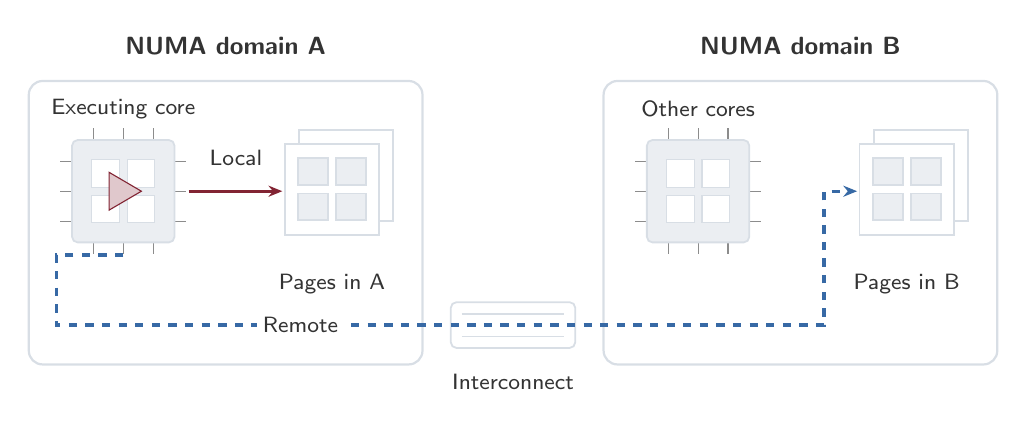
\begin{tikzpicture}[
 font=\small\sffamily,text=black!80,
 hardware/.style={draw=tabline,fill=neutralcol,line width=0.65pt},
 local/.style={-{Stealth[length=5pt,width=4pt]},draw=figcol,line width=1.2pt},
 remote/.style={-{Stealth[length=5pt,width=4pt]},draw=ddrcol,dashed,line width=1.2pt},
 note/.style={font=\footnotesize\sffamily,align=center},
 heading/.style={font=\small\sffamily\bfseries}
]
\foreach \xmin/\xmax/\mid/\name in {0/5/2.5/A,7.3/12.3/9.8/B} {
 \draw[draw=tabline,rounded corners=5pt,line width=0.8pt]
  (\xmin,0) rectangle (\xmax,-3.6);
 \node[heading] at (\mid,0.45) {NUMA domain \name};
}

% Core symbols; the first core is the highlighted access initiator.
\foreach \cx in {1.2,8.5} {
 \begin{scope}[shift={(\cx,-1.4)}]
  \foreach \p in {-0.38,0,0.38} {
   \draw[draw=black!45] (\p,-0.65)--(\p,-0.8);
   \draw[draw=black!45] (\p,0.65)--(\p,0.8);
   \draw[draw=black!45] (-0.65,\p)--(-0.8,\p);
   \draw[draw=black!45] (0.65,\p)--(0.8,\p);
  }
  \draw[hardware,rounded corners=2pt] (-0.65,-0.65) rectangle (0.65,0.65);
  \foreach \dx in {-0.4,0.05} \foreach \dy in {-0.4,0.05}
   \draw[draw=tabline,fill=white] (\dx,\dy) rectangle ++(0.35,0.35);
 \end{scope}
}
\draw[draw=figcol,fill=figcol!25] (1.02,-1.64)--(1.02,-1.16)--(1.43,-1.4)--cycle;
\node[note] at (1.2,-0.35) {Executing core};
\node[note] at (8.5,-0.35) {Other cores};

% Generic physical pages: the comparison is locality, not HBM versus DDR.
\foreach \cx/\name in {3.85/A,11.15/B} {
 \begin{scope}[shift={(\cx,-1.4)}]
  \draw[hardware,fill=white] (-0.42,-0.38) rectangle (0.78,0.78);
  \draw[hardware,fill=white] (-0.6,-0.56) rectangle (0.6,0.6);
  \foreach \dx in {-0.43,0.05} \foreach \dy in {-0.37,0.08}
   \draw[hardware] (\dx,\dy) rectangle ++(0.38,0.34);
 \end{scope}
 \node[note] at (\cx,-2.58) {Pages in \name};
}

% Local requests stay in A. Remote requests traverse a domain interconnect.
\draw[local] (2.03,-1.4)--(3.22,-1.4);
\node[note] at (2.63,-0.98) {Local};
\draw[hardware,fill=white,rounded corners=2pt]
 (5.36,-3.39) rectangle (6.94,-2.81);
\foreach \dy in {-3.24,-2.96}
 \draw[draw=tabline] (5.5,\dy)--(6.8,\dy);
\draw[remote] (1.2,-2.21)--(0.35,-2.21)--(0.35,-3.1)
 --(10.1,-3.1)--(10.1,-1.4)--(10.52,-1.4);
\node[note,fill=white,inner sep=2pt] at (3.45,-3.1) {Remote};
\node[note] at (6.15,-3.82) {Interconnect};
\end{tikzpicture}%
}
\endgroup

\caption{Local and remote NUMA access from a core in domain A.  Local
access targets pages in A; remote access reaches pages in B through an
interconnect.  The additional path and resource contention can change
latency and attainable bandwidth, without a universal numerical penalty.
Domains can lie within one socket or across sockets.  Arrows indicate
access requests; CPU caches and memory controllers are omitted to focus
on locality.  Page symbols do not identify a particular memory tier.}
\label{fig:numa-access-paths}
\end{figure}
\FloatBarrier

\textbf{Thread affinity} determines where threads execute; memory policy
influences which domains provide pages.  They are separate controls.
For ordinary anonymous allocations under a local default policy,
physical pages are commonly established on first touch rather than when
a virtual range is merely reserved.  Parallel initialization can thus
produce different locality from serial initialization.  Binding or
interleaving policies change allocation behavior, and file-backed mappings
have their own policy rules~\cite{linuxnumapolicy2026}.  Touching a tensor
on one core does not guarantee that later accesses by all other cores
are local.  Observed page placement and the loading mechanism must
support such a claim.

\textbf{Placement} describes where backing storage resides.
\textbf{Access traffic} describes bytes transferred while using it.
\textbf{Migration} changes existing data's residency, for example by
moving pages between domains.  Allocating a destination and copying
into it creates additional traffic and may temporarily require both
copies.  Cache-line fills do not by themselves constitute migration of
the tensor's backing pages.  These distinctions apply to both weight
and KV storage, independent of which policies a later design examines.

A cluster connects independently booted nodes and allocates them
through a scheduler.  Shared-memory access within a node differs from
explicit communication between nodes.  The actual topology, scheduler
workflow and operating conditions are developed in the platform and
methodology material.
\FloatBarrier

\section{Memory requirements and performance models}
\label{sec:performance-background}
\label{sec:memory-requirements}

\subsection{Weight, KV and workspace capacity}

\tabref{tab:inference-data} compares the main data classes.  Their
lifetimes explain why process memory does not simply follow a request's
context length.  Persistent weights, reusable KV pools and temporary
workspaces can coexist even when only part of the pool is populated.

\begin{table}[htbp]
\centering
\small
\tabsetup
\begin{tabularx}{\textwidth}{P{2.1cm}YYY}
\headrow
\headcell{Property} & \headcell{Weights} & \headcell{KV state} & \headcell{Temporary data} \\[3pt]
\tabheadrule
\tabstripeRow
Origin & Learned parameters & Per-layer keys and values computed from inputs & Intermediate results and kernel scratch space \\[3pt]
\tabrowsep
\tabplainRow
Lifetime & Model residency, often many requests & Needed history; pool can outlive requests & Operation or phase; allocation can be reused \\[3pt]
\tabrowsep
\tabstripeRow
Modification & Normally read-only after preparation & New entries written; history read & Written and consumed during computation \\[3pt]
\tabrowsep
\tabplainRow
Sharing & Shared by requests using the same representation & Per sequence logically; compatible prefixes can share blocks & Usually tied to current execution; buffers can be reused \\[3pt]
\tabrowsep
\tabstripeRow
Size drivers & Parameter count, types, format, packing, copies & Layers, KV heads, head size, retained positions, type, pool policy & Batch, prompt chunk, operator, implementation \\[3pt]
\tabrowsep
\tabplainRow
Access & Dense transforms reuse matrix tiles; embeddings select rows & Append state and read permitted history & Short-lived reads and writes; fusion can reduce materialization \\[3pt]
\tabbottomrule
\end{tabularx}
\caption{Origins, storage roles and access behavior of inference data.
A logical lifetime does not imply immediate deallocation or page eviction.}
\label{tab:inference-data}
\end{table}
\FloatBarrier

For \(N\) distinct stored parameters, uniform payload size \(s_W\)
bytes per parameter, and representation overhead \(M_{\mathrm{format}}\),
a weight representation occupies approximately
\begin{equation}
\label{eq:weight-payload}
 M_W \approx Ns_W + M_{\mathrm{format}}.
\end{equation}
\eqcaption{Weight representation estimate.  Format overhead includes
quantization metadata, alignment and padding; additional runtime copies
are accounted for separately.}

With mixed tensor types, the payload term becomes
\(\sum_j N_j s_j\), counting shared storage once.  Packing overhead must
be included in the representation it affects.  A training checkpoint
may additionally contain optimizer state that inference does not need,
so checkpoint bytes need not equal the inference weight payload.

As an illustrative example, exactly \(8\times10^9\) parameters stored
in BF16 require \(16\times10^9\) payload bytes: 16\,GB or approximately
14.90\,GiB.  Four-bit storage gives an ideal payload of 4\,GB
(3.73\,GiB).  If that illustrative format also stores one two-byte scale
per 32 weights, the scales add 0.5\,GB, giving 4.5\,GB (4.19\,GiB)
before other metadata and padding.  This is an example format, not a
size claim for every four-bit model.  A retained second copy of the
BF16 representation would add another 16\,GB regardless of the file's
size.  Here GB denotes \(10^9\) bytes and GiB denotes \(2^{30}\) bytes;
KiB similarly denotes \(2^{10}\) bytes.

For \(L\) layers with uniform full-history attention, \(n_{\mathrm{KV}}\)
KV heads per layer, head dimension \(d_h\), and \(s_{\mathrm{KV}}\)
bytes per stored scalar, the live unshared KV payload is
\begin{equation}
\label{eq:kv-live-payload}
 M_{\mathrm{KV,live}}=
 2L n_{\mathrm{KV}}d_h s_{\mathrm{KV}}\sum_i S_i.
\end{equation}
\eqcaption{Live KV payload for independent, unshared sequences.  The
factor two counts keys and values; \(S_i\) is the number of evaluated
positions whose state is retained for sequence \(i\).}

The dimensions are layers times heads times scalars per head times
bytes per scalar times positions, hence bytes.  \(S_i\) counts cached
positions, not automatically every emitted token, since the final
output may not have been evaluated.  Nonuniform layers require summing
per-layer payloads; bounded histories, shared prefixes, quantization
metadata and padding require corresponding adjustments.  Occupied block
capacity rounds each independently allocated length to block boundaries.
Reserved pool capacity can be larger still.

For an illustrative 32-layer model with eight KV heads, \(d_h=128\)
and two-byte entries, each retained position occupies
\(2\times32\times8\times128\times2=131{,}072\) bytes, or 128\,KiB.
An 8{,}192-position history therefore holds 1\,GiB of live KV payload.
Thirty-two independent sequences of that length hold 32\,GiB.
Replacing eight KV heads with 32, while keeping the other assumptions,
multiplies these sizes by four; using one KV head divides them by eight.
The examples isolate architecture and workload effects, without assuming
a particular named model or allocator.

A capacity budget must include allocations that coexist:
\begin{equation}
\label{eq:inference-allocation-budget}
 M_{\mathrm{allocated}} \approx M_W+M_{\mathrm{copies}}+
 M_{\mathrm{KV,allocated}}+M_{\mathrm{workspace}}+M_{\mathrm{other}}.
\end{equation}
\eqcaption{A simultaneous allocation budget.  KV allocation includes
its allocated pool or buffers, so live KV payload must not be added a
second time.  Other storage includes runtime metadata and allocator overhead.}

Combining the illustrative BF16 weights with the 32 unshared histories
gives about 46.90\,GiB of weight and live-KV payload before workspace and
allocation overhead.  A reserved pool larger than the live state raises
the allocation budget.  Temporary conversion buffers can instead make
loading the peak-memory interval.  The sum describes allocated storage,
not necessarily resident pages or controller traffic; neither logical
payload formulas nor process RSS alone identify all these components.

\subsection{Reuse and access traffic}

For the dense operation in \eqnref{eq:weights-activations}, there are
approximately \(2m d_{\mathrm{in}}d_{\mathrm{out}}\) floating-point
operations.  If its weight matrix is fetched once across the memory
boundary, weight traffic is \(s_W d_{\mathrm{in}}d_{\mathrm{out}}\)
bytes.  Neglecting all other traffic then gives the illustrative ratio
\(2m/s_W\) FLOP/byte.  It is a weight-only estimate: input and output
traffic, packing, cache reuse between evaluations and repeated tile
loads determine the actual arithmetic intensity.  Quantized kernels
also require a suitable operation-count convention.

Prefill and batches with several evaluated positions can reuse a weight
tile across activation rows.  Low-batch decode offers less of this
reuse, while longer histories increase attention's KV reads.  Distinct
sequences generally access distinct histories, although grouped heads,
shared prefixes and kernel tiling can allow further reuse.  Temporary
buffers can contribute significant traffic when intermediate results
are materialized.  Neither weights nor KV state should therefore be
declared universally dominant: the relevant balance depends on the
model, representation, phase, workload and memory boundary.

An estimated logical read of \(D\) bytes is not a measurement of
main-memory traffic.  Cache hits, writeback, prefetching and transfers
between locality domains alter the observed byte counts.  If some data
resides in HBM and some in DDR, their separate traffic and available
paths must be considered.  A single bandwidth ceiling cannot simply
be applied to the sum of both tiers' capacities.  Simultaneous transfers
may overlap, but they can also share compute resources or interconnects.
Migration adds its own reads, writes, synchronization and possible
capacity peak; a benefit must cover these costs over the interval in
which the new placement is used.

\subsection{Compute throughput and practical ceilings}

\textbf{Compute throughput} counts operations per unit time.  Floating-point
rates use FLOP/s; a multiplication and addition count as two operations,
including when fused into one instruction.  Peak throughput depends on
active cores, clock frequency, supported instructions and precision.
It is distinct from inference throughput in tokens/s, since one token
requires many operations and accesses.

Peak specifications describe ideal conditions.  Microbenchmarks can
establish practical compute and bandwidth ceilings for a chosen
configuration, while application measurements show how much of that
capability is used~\cite{nerscroofline2026}.  The capacity, latency and
bandwidth distinctions in \secref{sec:cpu-memory-systems} remain important:
low bandwidth utilization alone does not establish a compute bottleneck.

\subsection{Bandwidth requires concurrency}
\label{sec:littles-law}

High bandwidth requires enough independent transfers to keep memory
busy.  Little's law relates sustained bandwidth \(B\), mean access
latency \(\tau\), and mean bytes in flight \(C\):
\begin{equation}
\label{eq:little}
 C=B\tau.
\end{equation}
\eqcaption{Mean memory concurrency required in steady state.  Bytes/s
multiplied by seconds gives bytes in flight.}

Dividing \(C\) by cache-line size gives the corresponding outstanding
line count.  Finite per-core tracking resources limit how many misses
can overlap.  More cores, independent software accesses and prefetching
can supply additional requests, subject to those limits.  Use loaded
latency: queueing near saturation can raise it above idle latency, so an
idle measurement gives only an optimistic concurrency requirement.
Regular streams can expose this parallelism; dependent load chains may
not.  \secref{sec:platform-concurrency} applies the relationship to the
experimental platform.  This memory-request concurrency differs from
both active inference requests and execution-batch size.

\subsection{Reading a Roofline plot}
\label{sec:roofline}

The Roofline model relates a kernel's operation count to its data
movement~\cite{williams2009roofline}.  Let \(F\) be the number of
floating-point operations and \(D\) the bytes read and written across
the memory boundary being analysed.  Their ratio is the
\textbf{arithmetic intensity}:

\begin{equation}
\label{eq:arithmetic-intensity}
  I = \frac{F}{D}
  \qquad \text{[FLOP/byte]}.
\end{equation}
\eqcaption{Arithmetic intensity: the amount of computation performed
per byte transferred.}

For a main-memory Roofline, \(D\) counts traffic between main memory and
the cache hierarchy, rather than every access issued by the processor.
Reusing data in cache can reduce this traffic and increase \(I\).
If the computation takes time \(t\), its measured compute throughput is
\(P=F/t\), and its achieved bandwidth at that boundary is \(D/t\).

With a compute ceiling \(P_{\max}\) and bandwidth ceiling
\(B_{\max}\), the model gives

\begin{equation}
\label{eq:roofline}
  P \leq \min\!\left(P_{\max},\, B_{\max} I\right).
\end{equation}
\eqcaption{The Roofline bound: attainable throughput is limited by
both the processor's arithmetic rate and the supply of data.}

\figref{fig:roofline} plots this bound on logarithmic axes.  The
sloping part is the bandwidth limit \(B_{\max}I\); the horizontal
part is the compute limit \(P_{\max}\).  They meet at the
\textbf{ridge point}, whose intensity is
\(I_{\mathrm{ridge}}=P_{\max}/B_{\max}\).

\begin{figure}[htbp]
\centering
\begingroup
\definecolor{roofink}{HTML}{263445}
\definecolor{roofblue}{HTML}{365D85}
\colorlet{roofaccent}{sapred}
\definecolor{roofborder}{HTML}{CBD5DF}
\resizebox{\textwidth}{!}{%
\begin{tikzpicture}[
  font=\small\sffamily, text=roofink,
  axis/.style={-{Stealth[length=5pt,width=4pt]},
               draw=roofink!80, line width=0.8pt},
  note/.style={font=\footnotesize\sffamily, align=center},
  card/.style={draw=roofborder, fill=roofink!3, rounded corners=4pt,
               line width=0.65pt, inner xsep=7pt, inner ysep=7pt,
               text width=4.3cm, minimum height=2.5cm, align=left,
               font=\footnotesize\sffamily}
]
  % x = 3 log10(I / 0.1); y = 1.5 log10(P / 10).
  % Illustrative ceilings: 100 GB/s and 1000 GFLOP/s; ridge at 10 FLOP/byte.
  \fill[roofblue!7] (0,0) -- (6,3) -- (6,0) -- cycle;
  \fill[roofaccent!7] (6,0) rectangle (9,3);
  \foreach \x in {3,6,9}
    \draw[roofborder, line width=0.4pt] (\x,0) -- (\x,3.35);
  \foreach \y in {1.5,3}
    \draw[roofborder, line width=0.4pt] (0,\y) -- (9,\y);

  \draw[axis] (0,0) -- (9.45,0);
  \draw[axis] (0,0) -- (0,3.8);
  \foreach \x/\value in {0/0.1,3/1,6/10,9/100}
    \draw[roofink!70] (\x,0) -- (\x,-0.08)
      node[below, font=\footnotesize\sffamily] {\value};
  \foreach \y/\value in {0/10,1.5/100,3/{1{,}000}}
    \draw[roofink!70] (0,\y) -- (-0.08,\y)
      node[left, font=\footnotesize\sffamily] {$\value$};
  \node[note, rotate=90] at (-1.15,1.75)
    {Compute throughput $P$ [GFLOP/s]};
  \node[note] at (4.5,-0.65)
    {Arithmetic intensity $I$ [FLOP/byte]};

  \draw[roofaccent!55, densely dashed, line width=0.7pt]
    (0,3) -- (6,3);
  \draw[roofblue, line width=1.9pt] (0,0) -- (6,3)
    node[pos=0.58, sloped, above=4pt, note, text=roofblue]
      {Bandwidth limit: $B_{\max} I$};
  \draw[roofaccent, line width=1.9pt] (6,3) -- (9,3)
    node[midway, above=4pt, note, text=roofaccent]
      {Compute limit: $P_{\max}$};

  \draw[roofink!60, densely dashed] (6,0) -- (6,3);
  \fill[roofink] (6,3) circle (2.3pt);
  \node[note, anchor=south] (ridge) at (5.3,3.6)
    {Ridge point: $I_{\mathrm{ridge}}=P_{\max}/B_{\max}$};
  \draw[roofink!65, -{Stealth[length=4pt,width=3pt]}]
    (ridge.south) -- (6,3.08);

  \node[note, text=roofblue, font=\small\sffamily\bfseries]
    at (2.65,4.35) {Memory-bound region};
  \node[note, text=roofaccent, font=\small\sffamily\bfseries]
    at (7.6,4.35) {Compute-bound region};

  % Points are illustrative measurements below the roof.
  \draw[roofink!60, densely dashed] (3,1.05) -- (3,1.5);
  \fill[roofink] (3,1.05) circle (2.6pt);
  \node[note, anchor=north west] at (3.1,1.0) {Kernel A};
  \draw[roofink!60, densely dashed] (7.8,2.6) -- (7.8,3);
  \fill[roofink] (7.8,2.6) circle (2.6pt);
  \node[note, anchor=north] at (7.8,2.45) {Kernel B};

  \node[card, draw=roofblue!45, fill=roofblue!4] at (2.2,-2.3)
    {\textbf{Left of the ridge}\\
     Limited by data movement.\\
     More bandwidth lifts the roof.\\
     Reuse moves a kernel right.};
  \node[card, draw=roofaccent!45, fill=roofaccent!4] at (7.2,-2.3)
    {\textbf{Right of the ridge}\\
     Limited by arithmetic.\\
     Better use of compute units\\
     brings a kernel closer to the roof.};
\end{tikzpicture}%
}
\endgroup
\caption{A Roofline plot with illustrative ceilings of 100\,GB/s and
1{,}000\,GFLOP/s, giving a ridge at 10\,FLOP/byte.  Both axes are
logarithmic.  The sloping segment is the bandwidth limit and the
horizontal segment is the compute limit.  The roof is an upper
bound; the dots represent example kernel measurements below it, and the
dashed vertical segments show their gap to the bound.  This is a
conceptual example, not a measurement of the thesis platform.}
\label{fig:roofline}
\end{figure}

Left of the ridge, the model identifies a \textbf{memory-bound}, more
specifically bandwidth-bound, region.  Increasing bandwidth raises the
bound, while reusing each transferred byte more often moves a kernel to
the right.  Right of the ridge, the bound is \textbf{compute-bound};
additional bandwidth alone does not raise it.  For example, with the
figure's ceilings, intensity \(1\) limits throughput to 100\,GFLOP/s,
whereas intensity \(20\) permits at most 1{,}000\,GFLOP/s.

A point below the roof does not establish the cause of the gap.
Latency, limited parallelism, inefficient instructions and runtime overhead
can all reduce performance.  Compare kernels with ceilings for the same
cores, precision and memory boundary~\cite{nerscroofline2026}; integer
kernels require matching integer-operation counts and ceilings, not FLOP/s.

Prefill's weight reuse and low-batch decode's smaller reuse motivate
separate phase analysis.  Their actual intensity depends on batching,
history length, representation and kernels~\cite{na2024llmcpu}.
Roofline describes numerical work; request timing also includes scheduling
and other runtime overhead.
\FloatBarrier

%======================================================================
%  Common request and engine performance measurements
%======================================================================

\section{Performance metrics}
\label{sec:metrics}

Latency describes waiting and output pace; throughput describes a
processing rate.  \tabref{tab:inference-metrics} defines the loading,
phase and request measurements used to interpret inference~\cite{vllm2026}.
Their timing boundaries must be specified explicitly.

Comparisons state model, precision, prompt and output lengths, concurrency,
execution-batch limits and scheduling.  More concurrency can improve
aggregate throughput while increasing waiting.  The median describes
typical latency; p95 is the value at or below which 95\% of observations
fall.  Specify whether observations are requests, per-request averages,
or token intervals.  Memory footprint and hardware activity help explain
results; representation changes also require evaluating numerical quality.

\begin{table}[htbp]
\centering
\small
\tabsetup
\begin{tabularx}{\textwidth}{P{2.7cm}P{1.6cm}Y}
\headrow
\headcell{Metric} & \headcell{Unit} & \headcell{Meaning} \\[3pt]
\tabheadrule
\tabstripeRow
Model loading time
  & ms or s
  & Time from starting model preparation to a declared ready state;
    report whether page population, conversion and packing are included. \\[3pt]
\tabrowsep
\tabplainRow
Time to first token (TTFT)
  & ms or s
  & Time from the declared request start to the first output token.
    Describes the wait before generation becomes visible. \\[3pt]
\tabrowsep
\tabstripeRow
Inter-token latency (ITL)
  & ms
  & Time between successive output tokens.  Describes the pace and
    variability of generation. \\[3pt]
\tabrowsep
\tabplainRow
Time per output token (TPOT)
  & ms/token
  & Mean time per output token after the first, within one request.
    Summarises the generation interval. \\[3pt]
\tabrowsep
\tabstripeRow
End-to-end latency
  & ms or s
  & Time from the declared request start to its completion.
    Describes the wait for the full response. \\[3pt]
\tabrowsep
\tabplainRow
Prefill throughput
  & tokens/s
  & Prompt tokens processed per second of prompt evaluation, using a
    direct phase timer. \\[3pt]
\tabrowsep
\tabstripeRow
Output throughput
  & tokens/s
  & Generated tokens per second over a stated interval, for one
    sequence or aggregated across requests. \\[3pt]
\tabbottomrule
\end{tabularx}
\caption{Common inference performance metrics.  Smaller latency and
larger throughput indicate better performance under otherwise
comparable workloads.}
\label{tab:inference-metrics}
\end{table}
\FloatBarrier

For a request producing \(O>1\) tokens, let \(t_1\) and \(t_O\)
be the times of the first and last output tokens.  Then

\begin{equation}
\label{eq:tpot}
  T_{\mathrm{TPOT}} = \frac{t_O-t_1}{O-1}.
\end{equation}
\eqcaption{Mean generation time per output token, excluding the first.}

With one token per emission event, TPOT averages a request's ITL
intervals; streamed chunks instead measure delivery of several tokens~\cite{vllm2026}.
TPOT is undefined for one-token responses.  Its reciprocal gives the
post-first-token rate when measured in seconds/token, or
\(1000/T_{\mathrm{TPOT}}\) for milliseconds/token.  Aggregate throughput
is not the reciprocal of one request's TPOT; serving rate can also be
reported in completed requests/s.

TTFT can include queueing, input preparation, prefill and delivery,
according to the declared client or engine boundary~\cite{agrawal2025evaluating}.
The first output normally follows prefill, without an extra decode
evaluation.  Direct phase timers specify whether scheduling, cache
management, sampling and synchronization are included.  Decode throughput
counts evaluated positions, whereas output throughput counts emitted
tokens; ordinary generation produces its first output from prefill logits.

Report model loading and warm-up separately from steady-state inference,
including readiness and page-population conditions.  Warm-up can involve
page faults, kernel preparation and initial allocation.  Aggregate output
throughput divides emitted tokens by a declared observation duration,
with explicit treatment of warm-up, unfinished requests and interval
endpoints.  Client and engine timestamps require consistent boundaries.


\cleardoublepage

\chapter{Experimental Platform}
\label{chap:experimental-platform}

The preceding chapter described what the Xeon Max platform can support.
This chapter records the documented CRESCO8 configuration, distinguishes
documentation from observations that must be captured on the allocated
nodes, and states the constraints that the platform imposes on the study.

%======================================================================
%  CRESCO8: the cluster and the observed configuration of its HBM nodes
%======================================================================

\section{CRESCO8}
\label{sec:cresco8}

CRESCO8 is an ENEA compute system at the Portici research centre, in
service since 2025~\cite{cresco8doc,eneapress}.  It has three classes of
compute node (\tabref{tab:cresco8-node-classes}).  This thesis uses the
CPU--HBM class; the general CPU class matters only as a possible
system-level baseline.

\begin{table}[htbp]
\centering
\footnotesize
\tabsetup
\begin{tabularx}{\textwidth}{P{1.55cm}P{1.05cm}P{1.45cm}P{2.65cm}Y}
\headrow
\headcell{Class} & \headcell{Nodes} & \headcell{CPU cores}\newline\headcell{per node}
 & \headcell{Memory}\newline\headcell{per node} & \headcell{Processor or accelerator} \\[3pt]
\tabheadrule
\tabstripeRow
CPU
 & 760 & 128 & 512\,GB DDR5
 & 2$\times$ Xeon Platinum 8592+ \\[3pt]

\tabrowsep
\tabplainRow
CPU--HBM
 & 16 & 112 & 1{,}024\,GB DDR5\newline + 128\,GB HBM
 & 2$\times$ Xeon CPU Max 9480 \\[3pt]

\tabrowsep
\tabstripeRow
GPU
 & 17 & 128 & 512\,GB DDR5\newline + accelerator HBM
 & 2$\times$ Xeon Platinum 8592+ and
   4$\times$ Intel Data Center GPU Max 1550 \\[3pt]
\tabbottomrule
\end{tabularx}
\caption{CRESCO8 node classes.  The CPU and GPU rows follow the ENEAGRID
documentation~\cite{cresco8doc}.  The CPU--HBM count is the scheduler's:
on 11 October 2026 Slurm listed 16 HBM nodes, whereas the documentation
lists 15.}
\label{tab:cresco8-node-classes}
\end{table}

The general CPU nodes are not a clean control for the HBM nodes.  The
Platinum 8592+ is an Emerald Rapids processor, one generation newer than
the Max 9480, with 64 cores, DDR5-5600 memory and a 320\,MB last-level
cache, nearly three times the Max 9480's 112.5\,MB~\cite{intel8592}.  A
comparison between the two node classes changes the core count, the
memory speed and the cache size together with the absence of HBM.  The
cache difference is the most serious confound for inference: the weights
of a model of a few hundred million parameters at 4-bit precision fit
almost entirely in the 8592+'s cache, which is the cache-residency effect
that Zhang et al.\ exploit~\cite{zhang2026cacheresident}.  Such a
comparison is therefore reported, if at all, as a system-level baseline
and never as an HBM effect.

\subsection{Interconnect}

Each HBM node has an NVIDIA ConnectX-7 adapter with one InfiniBand port
active at 200\,Gb/s, the NDR200 rate.  That is 25\,GB/s in each
direction: about a fortieth of one socket's nominal HBM bandwidth and a
twelfth of its DDR5 interface peak (\tabref{tab:xeon-max-peaks}).
Distributing a model
across nodes would make the network, not the memory tier, the dominant
cost, which is one reason the experiments stay within one node.

\subsection{Scheduler and allocation policy}
\label{sec:cresco8-scheduler}

Compute nodes are reached only through Slurm; the front-end nodes are
for editing, compilation and submission, not for measurement.  The HBM
nodes are split between two partitions with disjoint node lists.
\texttt{cresco8\_hbm} contains \texttt{cresco8-hbm01} to \texttt{hbm14},
with a 24-hour limit and a quality-of-service limit of five nodes per
user.  \texttt{cresco8\_hbm\_dbg} contains \texttt{hbm15} and
\texttt{hbm16}, with a one-hour limit.

The scheduler (Slurm 25.11.8) allocates individual cores
(\texttt{select/cons\_tres} with \texttt{CR\_CORE}) and does not allow jobs
of different users to be excluded from a node unless a job asks for it.
Without \texttt{-{}-exclusive}, another user's job can therefore run on the
other cores of the same node and compete for the same memory bandwidth
and, in Cache mode, the same HBM cache.  Every measurement in this thesis
uses an exclusive allocation.  Jobs run inside cgroup-v2 containers with
core and memory confinement: a job may use only the memory it requests,
and 10\,GB per node are reserved for the system.  The memory set of the
cgroup, by contrast, is not restricted (\secref{sec:hbm-clustering}).

\subsection{Storage and model staging}
\label{sec:cresco8-storage}

ENEAGRID provides AFS for home directories and the Lustre file system
\texttt{/lpor1}, 6.9\,PB in size and 90\% occupied at the time of the
check, for parallel I/O~\cite{cresco8doc}.  Each HBM node also has a
960\,GB Micron 7450 NVMe drive.  It holds the operating system, and its
root file system, including \texttt{/tmp}, had 104\,GB free; Slurm does
not manage it as a resource.  \texttt{/dev/shm} is a memory-backed file
system of up to 504\,GB.

Where the model file lives affects the measurement.  Runtimes such as
\lcpp{} map the model file into memory by default, so the weights become
page-cache pages of a Lustre file.  Those pages can be evicted and fetched
again over the network during a run, and their placement is decided when
they are first read rather than by the experiment's binding.  Models are
therefore staged to node-local storage before a run, and the weights are
loaded into anonymous memory (for \lcpp{} with \texttt{-{}-no-mmap}) so
that the binding applies to them.  The staging method is recorded with
each result.

\subsection{Software environment}
\label{sec:cresco8-software}

The HBM nodes run Red Hat Enterprise Linux~9.4 with kernel
5.14.0-427.13.1.  The kernel is booted with \texttt{mitigations=off} and
\texttt{intel\_pstate=disable}, and a site-specific \texttt{tuned}
profile is active.  The system compiler is GCC~11.4.1.  Environment
modules provide GCC~12, 14 and 15.1 and the Intel oneAPI 2025, 2025.3
and 2026.1 toolchains; oneAPI and an Intel-built Open MPI are loaded at
login by default.  \texttt{hwloc}~2.4.1 and \texttt{numactl} are
installed.  The versions of the inference runtimes and their libraries
are fixed per experiment, as described in the methodology.

\subsection{Observed configuration of the HBM nodes}
\label{sec:cresco8-observed}

The configuration of the regular HBM partitions was captured on
\texttt{cresco8-hbm15} by an exclusive job on 11 October 2026, with the
probes listed in \appref{app:reproducibility}.  The same probes are part
of the platform record that the benchmark suite stores with every
campaign~\cite{hwbench2026}, so each measurement in the following
chapters carries its own copy of this table.  An earlier allocation on
the same node, on 29 September 2026, had already shown two NUMA nodes and
no separate HBM node.  \tabref{tab:cresco8-manifest} lists what was
observed and why each item matters for the experiments.

\begin{table}[htbp]
\centering
\small
\tabsetup
\begin{tabularx}{\textwidth}{P{2.7cm}P{5.0cm}Y}
\headrow
\headcell{Item} & \headcell{Observed} & \headcell{Consequence} \\[3pt]
\tabheadrule
\tabstripeRow
Memory mode
  & Cache: two NUMA nodes of 503\,GB, each behind a 64\,GiB direct-mapped,
    write-back memory-side cache with 64\,B lines
  & HBM use is decided by footprint and physical placement, not by
    binding. \\[3pt]

\tabrowsep
\tabplainRow
Clustering
  & Quadrant: one NUMA node per socket
  & Binding is per socket. \\[3pt]

\tabrowsep
\tabstripeRow
DDR5 population
  & Eight 64\,GB DIMMs per socket, one per channel
  & All eight channels available. \\[3pt]

\tabrowsep
\tabplainRow
Threads
  & SMT inactive; 112 logical CPUs, one per core
  & Thread count equals core count. \\[3pt]

\tabrowsep
\tabstripeRow
Frequency control
  & \texttt{acpi-cpufreq} driver, \texttt{schedutil} governor
  & Frequency is not fixed; it is sampled during runs. \\[3pt]

\tabrowsep
\tabplainRow
NUMA balancing
  & Disabled; memory-tier demotion disabled
  & The kernel does not migrate pages behind the experiment. \\[3pt]

\tabrowsep
\tabstripeRow
Zone reclaim
  & \texttt{zone\_reclaim\_mode} = 1
  & A full local node reclaims page cache before allocating remotely. \\[3pt]

\tabrowsep
\tabplainRow
Huge pages
  & Transparent huge pages \texttt{always}; defragmentation on
    \texttt{madvise}
  & Large allocations get 2\,MB pages when free memory allows. \\[3pt]

\tabrowsep
\tabstripeRow
Counters and energy
  & \texttt{perf\_event\_paranoid} = 2; no \texttt{perf}; MSR and RAPL
    readable by root only
  & No uncore traffic or RAPL energy for users
    (\secref{sec:sd650-node}). \\[3pt]

\tabrowsep
\tabplainRow
Job cgroup
  & \texttt{cpuset.mems.effective} = \texttt{0-1}
  & Memory binding is not restricted by Slurm. \\[3pt]
\tabbottomrule
\end{tabularx}
\caption{Configuration of a CRESCO8 HBM node as observed by an exclusive
job on \texttt{cresco8-hbm15}, 11 October 2026.}
\label{tab:cresco8-manifest}
\end{table}

\figref{fig:cresco8-lstopo} is the topology reported by \texttt{lstopo}
on the same node.  It confirms the Cache-mode picture: each package has
one NUMA node of about 503\,GB, and the 64\,GB HBM appears only as a
\texttt{MemCache} object in front of it, never as allocatable memory.

\paragraph{The Flat-mode node.}  In addition to the regular partitions,
one HBM node has been configured in Flat mode with Quadrant clustering
for this work and is reached outside the regular partitions.  Its NUMA
topology has the four nodes
expected from \tabref{tab:hbm-six-configurations}: two CPU-bearing DDR5
nodes of about 503\,GiB and two memory-only HBM nodes of 64\,GiB, one per
socket.  The firmware's distance from a socket's cores to its local HBM
node is 13, and to the other socket's HBM node 23~\cite{hwbench2026}.
Flat-mode placement experiments run on this node; the node identifiers
are read from the running system before each run rather than assumed.

\begin{figure}[htbp]
\centering
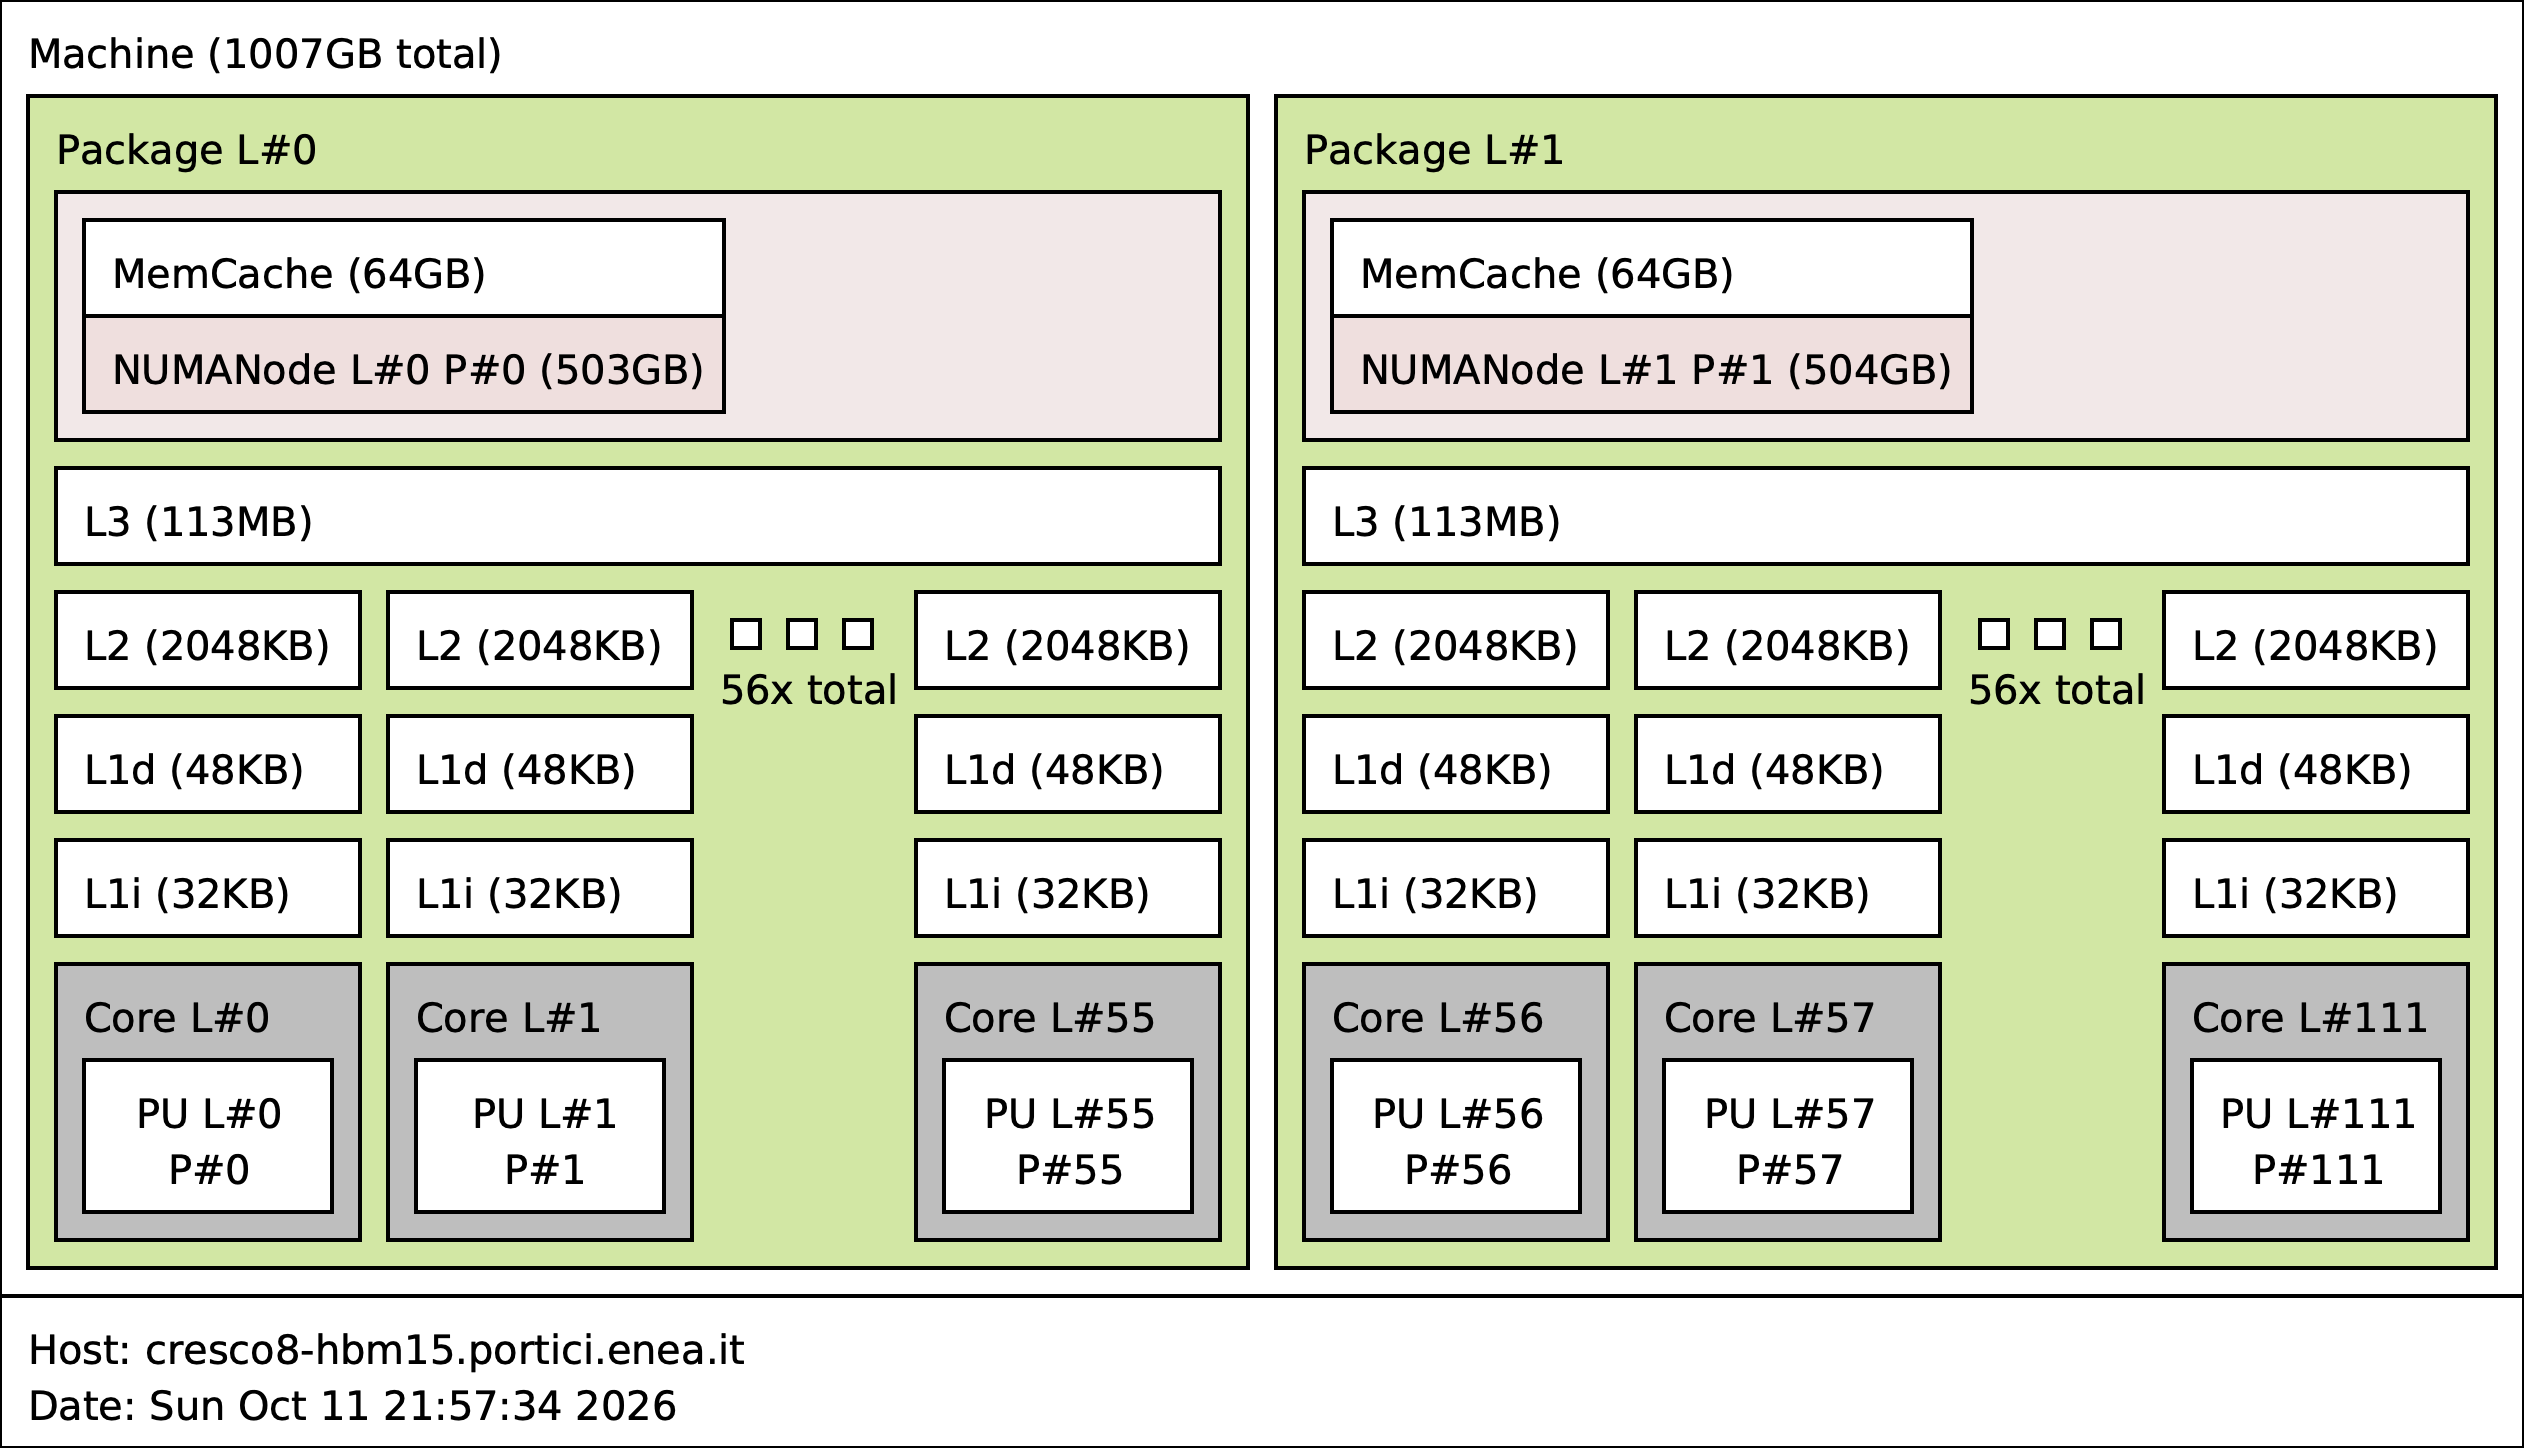
\includegraphics[width=0.9\textwidth]{cresco8-hbm-node-lstopo.png}
\caption{Topology of \texttt{cresco8-hbm15} as reported by
\texttt{lstopo} (hwloc~2.4.1) on 11 October 2026.  Two packages of 56
cores, each with a 113\,MB L3 and one DDR5 NUMA node behind a 64\,GB
memory-side cache (\texttt{MemCache}): the signature of Cache mode with
Quadrant clustering.}
\label{fig:cresco8-lstopo}
\end{figure}

\subsection{Why this platform}
\label{sec:why-cresco8}

Systems that combine HBM and DDR on a general-purpose CPU are rare, and
the largest, Aurora, is the source of most published measurements on the
Xeon Max~\cite{ibeid2025aurora,goto2026aurorahpl} but is not available to
this work.  CRESCO8's 16 HBM nodes provide access to the processor and
both of its local memories, and the experiments need only one socket at a
time.  The platform also sets a constraint.  Memory and clustering modes
are fixed at boot and the nodes are shared with other users, so the
configuration is not a per-job variable.  Two configurations are
available: Cache with Quadrant clustering on the regular partitions, and
Flat with Quadrant clustering on one dedicated node.  SNC4 and HBM-only
would each be a separate block of experiments arranged with the
administrators.


\cleardoublepage

\chapter{Methodology}
\label{chap:methodology}

This chapter converts the theoretical model into a provisional,
controlled empirical study.  The related-work synthesis and research
gap still require revision.  The design
separates outcome metrics, explanatory measurements, and validity checks.

%======================================================================
%  Focused experimental design
%======================================================================

\section{Focused experimental design}
\label{sec:methodology}

\subsection{Objective and research questions}

The working objective is to determine how the two local memory systems
of a Xeon Max socket can jointly serve LLM inference.  In Flat mode,
software can place weights and KV blocks in HBM or DDR5 and can schedule
work against both tiers.  In Cache mode, HBM is a hardware-managed cache
for DDR5, so the same object-level placement policies cannot be applied.
The questions in \tabref{tab:research-questions} are provisional until
the literature review and platform configuration have been checked.
The September 2026 CRESCO8 check found Cache mode.  Flat-mode
experiments therefore require an administrator-provided configuration;
the Cache-mode question remains executable on the observed nodes.

\begin{table}[htbp]
\centering
\small
\tabsetup
\caption{Provisional research questions and testable predictions.  The
predictions are expectations, not conclusions.}
\label{tab:research-questions}
\begin{tabularx}{\textwidth}{@{}lYY@{}}
\toprule
\headrow
 & \textbf{Question} & \textbf{Prediction} \\
\midrule
RQ1
 & Which inference phases and memory objects demand HBM bandwidth, DDR
   bandwidth, or capacity on one Max 9480 socket?
 & Weight traffic dominates some low-batch decode regimes, while KV
   traffic grows with context and concurrency.  Neither tier's STREAM
   ratio alone predicts end-to-end performance. \\
RQ2
 & In Flat mode, can concurrent HBM and DDR access outperform the best
   single-tier or static split policy at the same total core count?
 & A split helps only when work in both tiers overlaps enough to offset
   scheduling and reduction overhead; the result depends on traffic,
   bandwidth saturation and thread allocation. \\
RQ3
 & How should weights and KV blocks be placed as model size, context,
   concurrency and HBM capacity change?
 & Keeping repeatedly streamed weights in HBM may beat placing the
   entire KV pool there; the best allocation can change as KV traffic
   grows.  Adaptive placement must beat tuned static baselines. \\
\addlinespace[2pt]
RQ4
 & How does hardware Cache mode compare with Flat-mode policies for
   representative working sets, if both modes are available?
 & Cache mode may help when reuse fits its effective cache capacity;
   Flat mode may do better when software can divide bandwidth and
   capacity explicitly.  No ordering is assumed. \\
\bottomrule
\end{tabularx}
\end{table}

The current vLLM CPU-tiered-KV branch is an experimental implementation
for RQ2 and RQ3, not a result that establishes either prediction.  Its
weight-in-HBM, block-level KV split, feedback allocator and parallel
attention scheduler require separate ablations.  Energy per token is a
conditional outcome until a measurement interface has been validated.
Multi-node inference and GPU comparison are outside the minimum scope.


\subsection{Evidence and the primary contrast}

Four evidence levels should remain distinct:

\begin{enumerate}
  \item a product guide establishes what a platform \emph{can} support;
  \item ENEAGRID documentation establishes what the site reported at a
        stated date;
  \item the system manifest establishes what an allocated node exposed;
        and
  \item repeated measurements establish how a specified workload
        behaved.
\end{enumerate}

The first controlled contrast holds the processor, socket, cores,
executable, model and workload constant while changing verified page
placement between local HBM and local DDR5 in Flat mode.  It calibrates
the tier effect; it is not the whole thesis question.  The next contrast
uses the same total core count and memory budget to compare sequential
and concurrent access to both tiers, followed by object-level placement
policies.  A Flat--Cache comparison, if possible, is a comparison of
memory-management modes rather than an isolated tier effect.

\subsection{Experimental sequence}

The work should advance \emph{only} after the preceding stage is
stable, in the dependency order drawn in
\figref{fig:experimental-sequence}.

\begin{figure}[htbp]
\centering
\resizebox{\textwidth}{!}{%
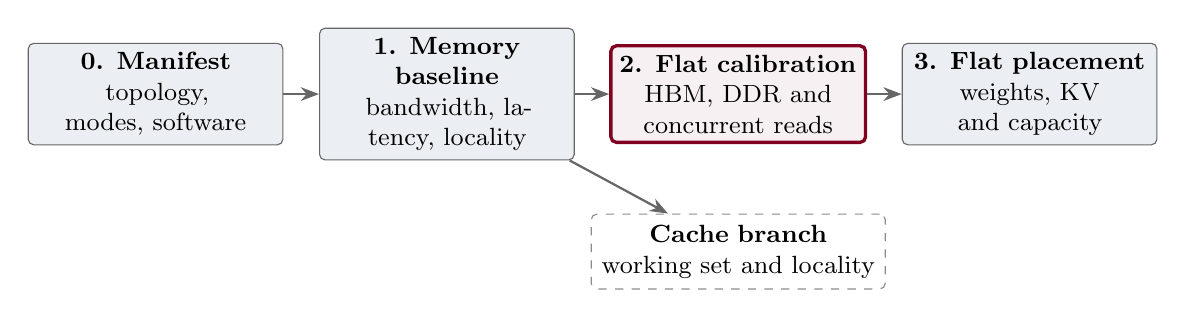
\begin{tikzpicture}[
  font=\small,
  stage/.style={draw=black!60, fill=neutralcol, rounded corners=2pt,
                text width=3.0cm, minimum height=1.15cm, align=center},
  primary/.style={stage, draw=accent, very thick, fill=accent!6},
  optional/.style={draw=black!45, dashed, fill=white, rounded corners=2pt,
                   text width=3.5cm, minimum height=0.95cm, align=center},
  flow/.style={-{Stealth}, thick, black!60}
]
  \node[stage] (s0) at (0,0)
    {\textbf{0. Manifest}\\topology, modes, software};
  \node[stage] (s1) at (3.7,0)
    {\textbf{1. Memory baseline}\\bandwidth, latency, locality};
  \node[primary] (s2) at (7.4,0)
    {\textbf{2. Flat calibration}\\HBM, DDR and concurrent reads};
  \node[stage] (s3) at (11.1,0)
    {\textbf{3. Flat placement}\\weights, KV and capacity};
  \node[optional] (s4) at (7.4,-2.0)
    {\textbf{Cache branch}\\working set and locality};

  \draw[flow] (s0) -- (s1);
  \draw[flow] (s1) -- (s2);
  \draw[flow] (s2) -- (s3);
  \draw[flow] (s1) -- (s4);
\end{tikzpicture}%
}
\caption{Proposed experimental dependency order.  Author's design.}
\label{fig:experimental-sequence}
\end{figure}

\begin{description}
  \item[Stage 0: system manifest.] Record the items in
  \tabref{tab:platform-record}, identify active memory and clustering
  modes, and request a Flat-mode block if available.  Only in Flat mode
  identify separate HBM and DDR NUMA nodes.

  \item[Stage 1: memory characterization.] Measure local and remote read,
  copy and triad bandwidth; unloaded and loaded latency; core-count
  scaling; and concurrent HBM--DDR traffic.  Establish saturation and
  run-to-run variability before fitting a performance model.

  \item[Stage 2: inference tier calibration, when Flat is available.]
  Freeze runtime commits,
  compiler and build.  Separate prefill from decode and compare verified
  local HBM and DDR placement.  Measure serial and concurrent access to
  both tiers with the same total core count and byte traffic.

  \item[Stage 3: object placement and capacity, when Flat is available.]
  Compare all-HBM where
  feasible, all-DDR, weights-first, KV-first and mixed-KV policies as
  context and concurrency grow.  Evaluate the existing vLLM branch
  against static allocation and attention-scheduling ablations, with
  residency and output checks.  Keep any \lcpp{} result as a separately
  named runtime baseline.

  \item[Cache-mode branch.] Measure the Cache-mode
  working-set transition on the observed nodes.  If Flat is also
  available under comparable conditions, compare modes explicitly.
  Without Flat, report Cache-mode results and leave RQ2--RQ3
  unanswered for CRESCO8 rather than implying tier control.
\end{description}

\subsection{Selecting factors without a Cartesian explosion}

The experiment matrix should be chosen from \textbf{hypotheses and
pilot data}, not by taking every combination of model, precision,
length, batch, core count and topology.  \tabref{tab:experimental-factors} lists the
factors that survive that test and states what each one is for.

\begin{table}[htbp]
\centering
\small
\tabsetup
\caption{Factors and the role of each in the experimental design.}
\label{tab:experimental-factors}
\begin{tabularx}{\textwidth}{@{}lYY@{}}
\toprule
\headrow
\textbf{Factor} & \textbf{Primary levels} & \textbf{Purpose} \\
\midrule
Memory placement
 & Local HBM, local DDR5, weights-first, KV-first and mixed KV
 & Isolate tier effects and test use of both bandwidth sources. \\
Working-set regime
 & Comfortably below, near, and above usable local HBM capacity
 & Locate a capacity boundary using measured resident memory rather than
   parameter count alone. \\
Precision
 & BF16 reference and at least one practical quantized weight format;
   KV precision recorded independently
 & Test whether reduced traffic, packing and kernel coverage change the
   HBM benefit. \\
Workload shape
 & Short and long prompt; short and sustained generation; low and
   moderate batch/concurrency
 & Separate prefill, weight-streaming decode and KV-dominant regimes. \\
Core/topology
 & Partial and full local socket; fixed total cores with varied HBM/DDR
   attention split; SNC4 only if available
 & Identify saturation, overlap and scheduling overhead. \\
Cache state
 & Cold-start/model-load and warmed steady state reported separately
 & Prevent file I/O or page-cache state from contaminating inference
   measurements. \\
\bottomrule
\end{tabularx}
\end{table}

Models should be selected by memory regime and architecture rather than
popularity alone.  The design should include a model/format that fits
comfortably in local HBM and one configuration close to the usable
capacity boundary.  At least one grouped-query model is useful because
its KV growth differs from full multi-head attention.  If the boundary
cannot be crossed with available models, context, concurrency or a
controlled allocation can be used to change the live set, provided the
mechanism does not alter the computation being compared.

Pilot runs determine the final numeric levels.  A sparse matrix of
representative points followed by focused sweeps around observed knees
is more informative than a large under-replicated grid.

\subsection{Runtime and correctness controls}

Use named, frozen commits of the experimental vLLM CPU branch for mixed
KV placement and of its unmodified base for runtime comparisons.  The
branch's present allocator assigns KV blocks to HBM or DDR for their
lifetime, and its decode path can process tier-local runs concurrently.
It does not migrate existing blocks.  Compare policies within the same
commit when possible so that allocator, kernel and model changes do not
confound the result.  A \lcpp{} run can calibrate broader CPU inference,
but its token rates are not a controlled baseline for a vLLM policy.

Performance comparisons are meaningful only when the computation is
equivalent.  Record the model revision and tokenizer, use fixed prompts
and seeds where supported, and validate token sequences or task-level
quality when precision changes.  If different kernels or quantization
formats change model quality, report that difference rather than
treating them as interchangeable.

\subsection{Metrics and explanatory measurements}

The metric definitions, equations and validity criteria are consolidated
in \secref{sec:metrics}; they are not repeated here.  The primary report
contains direct prompt-evaluation time, TTFT, the inter-token-latency
distribution, TPOT and output throughput at the declared concurrency.
Peak and steady resident memory are decomposed by object and tier where
the runtime and operating system expose that information.  Model loading
and tokenization remain outside the phase timings unless a separately
declared end-to-end experiment includes them.

The explanatory counter set is the smallest one able to test the proposed
mechanism: HBM and DDR traffic, UPI or remote traffic, achieved frequency,
cache misses and relevant matrix-engine activity.  Counter names and
availability are processor- and permission-specific.  A counter is
omitted rather than assigned a meaning that its scope does not support.
Throughput and reciprocal latency from the same synchronous batch are two
presentations of one observation, not independent confirmation.

\subsection{Run protocol and statistical analysis}

Each reported comparison should follow the same protocol:

\begin{enumerate}
  \item reserve an exclusive node and archive the system manifest;
  \item pin physical cores and memory explicitly, with SMT treated as a
        separate factor;
  \item verify page residency after model initialization and during the
        run, not only after allocation;
  \item separate model loading and warm-up from steady-state timing,
        unless they are part of the declared metric;
  \item counterbalance or randomize policy run order to reduce
        thermal and temporal bias;
  \item retain every raw sample, failure and outlier flag together with
        the command and environment;
  \item determine replication from pilot variability, using paired runs
        on the same node where possible; and
  \item repeat a subset on more than one HBM node before generalizing to
        the partition.
\end{enumerate}

Report absolute values and paired effect sizes, not only normalized bar
charts.  For primary comparisons, provide the median and interquartile
range together with a 95\% confidence interval appropriate to the
sampling design.  Tail percentiles require enough generated tokens or
requests to estimate them; p99 from a handful of observations is not a
tail-latency result.

The independent unit for a placement effect is a randomized or
counterbalanced policy run pair on a named node, not an individual
token.  Token latencies within one request share the same process,
machine state and autoregressive history and must not be counted as
independent replicates.  Confidence intervals therefore resample paired
runs (and, if the within-run distribution is analysed, preserve its
request-level grouping) rather than pooling every token into an
artificially large sample.

\subsection{Energy, if the boundary can be defended}

RAPL estimates processor-domain energy; XClarity/INA226 and a rack or
node power meter may cover different hardware.  Before reporting
joules/token, validate access, units, update rate, counter wraparound and
the components included in each source.  Integrate energy over the same
timed region as performance.  Gross joules/request and
joules/output-token should be reported; if idle energy is subtracted,
also report the gross value and the subtraction procedure.  Facility
cooling claims require a measured facility boundary and are outside a
node-level study.

\subsection{Threats to validity}

\tabref{tab:validity} pairs each class of threat with the design
feature that answers it.  The pairing matters more than the list: a
threat with no corresponding response is one the study cannot claim to
have addressed.

\begin{table}[htbp]
\centering
\small
\tabsetup
\caption{Main validity threats and design responses.}
\label{tab:validity}
\begin{tabularx}{\textwidth}{@{}lYY@{}}
\toprule
\headrow
\textbf{Validity} & \textbf{Threat} & \textbf{Response} \\
\midrule
Internal
 & Frequency drift, first touch, page migration, remote access, warm
   cache state or shared-node interference is mistaken for an HBM effect.
 & Exclusive nodes, paired order, explicit binding, residency checks and
   frequency/traffic measurements. \\
Construct
 & STREAM is treated as LLM bandwidth; file size as live memory; average
   TPOT as tail latency; RAPL as whole-node energy.
 & Define each metric and boundary, measure the live set, and use
   counters only to test a stated mechanism. \\
External
 & One model, precision, node or runtime is generalized to CPU inference
   as a whole.
 & Cover distinct memory regimes, repeat on multiple nodes, and state the
   platform/runtime boundary of every conclusion. \\
Statistical conclusion
 & Few repetitions, selected best runs or unreported failures inflate an
   effect.
 & Retain raw samples, predeclare primary comparisons and report
   uncertainty with absolute values. \\
Reproducibility
 & Modules, firmware, models and scheduler inventory change over time.
 & Archive immutable source/model revisions, build metadata, commands
   and dated system manifests. \\
\bottomrule
\end{tabularx}
\end{table}


\subsection{When an implementation contribution is justified}

The experimental vLLM branch already contains an object-level placement
implementation.  The present task is to determine whether its mixed KV
allocation and concurrent attention improve measured performance over
strong static baselines, and under which workloads.  Further policy
changes should target a measured inefficiency rather than be assumed
beneficial.

Compare all-local placement when it fits, weights-first and KV-first
tiering, static mixed fractions, the adaptive allocator, and the tier
attention scheduler both enabled and disabled.  Include placement and
reduction overhead, remote traffic, memory use and output quality.
Claim novelty only after the revised literature review and controlled
measurements establish what differs from prior tiered-attention work.


\cleardoublepage


% ================== APPENDICES ==================
\appendix
\chapter{Reproducibility Checklist}
\label{app:reproducibility}

This appendix records the operational material behind the observed
platform configuration in \secref{sec:cresco8-observed}.  It is
separated from the platform chapter because the commands support the
argument but are not part of it.  The hardware measurement campaigns,
with their kernels, scripts and raw records, and the platform record
described below are maintained in a separate repository, which is the
single source for both~\cite{hwbench2026}.

\section{Configuration probes}
\label{app:configuration-probes}

Every item of \tabref{tab:cresco8-manifest} is read by an ordinary user
inside an exclusive allocation, without root privileges, on the
execution node itself.  The benchmark suite's system snapshot performs
these reads at the start of every campaign and stores them as a
structured platform record next to the topology map, together with the
\texttt{lstopo} capture of \figref{fig:cresco8-lstopo}.
\tabref{tab:configuration-probes} lists the source of each item, so that
the observation can be repeated on any later date or node.

\begin{table}[htbp]
\centering
\small
\tabsetup
\begin{tabularx}{\textwidth}{P{3.0cm}Y}
\headrow
\headcell{Item} & \headcell{Command or kernel interface} \\[3pt]
\tabheadrule
\tabstripeRow
Topology
 & \texttt{lstopo}, \texttt{numactl -{}-hardware}, \texttt{lscpu},
   \texttt{lscpu -C} \\[3pt]

\tabrowsep
\tabplainRow
Memory-side cache
 & \texttt{/sys/devices/system/node/node*/\allowbreak memory\_side\_cache/\allowbreak index*/}
   \{\texttt{size}, \texttt{line\_size}, \texttt{indexing},
   \texttt{write\_policy}\} \\[3pt]

\tabrowsep
\tabstripeRow
DIMM population
 & \texttt{/sys/devices/system/edac/\allowbreak mc/mc*/dimm*/}\{\texttt{size},
   \texttt{dimm\_label}\} \\[3pt]

\tabrowsep
\tabplainRow
Threads and frequency
 & \texttt{/sys/devices/system/cpu/smt/active};
   \texttt{/sys/devices/system/cpu/cpu0/\allowbreak cpufreq/}\{\texttt{scaling\_driver},
   \texttt{scaling\_governor}\}; \texttt{/proc/cmdline} \\[3pt]

\tabrowsep
\tabstripeRow
Page policy
 & \texttt{/proc/sys/kernel/numa\_balancing},
   \texttt{/proc/sys/vm/zone\_reclaim\_mode},
   \texttt{/sys/kernel/mm/numa/demotion\_enabled},
   \texttt{/sys/kernel/mm/transparent\_hugepage/}\{\texttt{enabled},
   \texttt{defrag}\} \\[3pt]

\tabrowsep
\tabplainRow
Counters and energy
 & \texttt{/proc/sys/kernel/perf\_event\_paranoid};
   \texttt{/sys/class/powercap/intel-rapl:0/energy\_uj};
   \texttt{/dev/cpu/0/msr}; \texttt{scontrol show node} for Slurm's
   energy fields \\[3pt]

\tabrowsep
\tabstripeRow
Job cgroup
 & \texttt{cpuset.mems.effective} under the job's path in
   \texttt{/sys/fs/cgroup}, found from \texttt{/proc/self/cgroup} \\[3pt]

\tabrowsep
\tabplainRow
Network and storage
 & \texttt{ibstat}; \texttt{lsblk}; \texttt{df -hT} on \texttt{/tmp},
   \texttt{/dev/shm} and the Lustre mount \\[3pt]

\tabrowsep
\tabstripeRow
Scheduler
 & \texttt{sinfo}, \texttt{scontrol show partition},
   \texttt{scontrol show config}, \texttt{sacctmgr show qos} \\[3pt]
\tabbottomrule
\end{tabularx}
\caption{Sources of the observed configuration items.  All are readable
without root privileges; the RAPL and MSR entries are listed because
their \emph{unreadability} is the observation.}
\label{tab:configuration-probes}
\end{table}

\section{Minimum platform record}
\label{app:platform-record}

Each reported measurement carries, in addition, the record in
\tabref{tab:platform-record}.

\begin{table}[htbp]
\centering
\small
\tabsetup
\begin{tabularx}{\textwidth}{lY}
\headrow
\headcell{Category} & \headcell{Record} \\[3pt]
\tabheadrule
\tabstripeRow
Identity
 & Hostname, Slurm job ID, partition, date and node allocation. \\[3pt]

\tabrowsep
\tabplainRow
Processor
 & Exact SKU, sockets, physical cores, SMT state, microcode, governor
   and frequency sampled during the run. \\[3pt]

\tabrowsep
\tabstripeRow
Memory
 & Memory and clustering modes, NUMA distance matrix, HBM and DDR
   node IDs, huge-page state and verified page residency. \\[3pt]

\tabrowsep
\tabplainRow
I/O
 & Location of the model file and how it was loaded (staged copy,
   memory map or anonymous memory). \\[3pt]

\tabrowsep
\tabstripeRow
Software
 & OS and kernel, loaded modules, compiler, runtime commit, linked
   libraries, build flags and complete command line. \\[3pt]

\tabrowsep
\tabplainRow
Telemetry
 & Counter and energy interfaces used, with their permissions and
   measurement boundaries. \\[3pt]
\tabbottomrule
\end{tabularx}
\caption{Minimum platform record for an inference result.}
\label{tab:platform-record}
\end{table}

\section{Exposing HBM in Flat mode}
\label{app:flat-mode-setup}

Flat mode needs two configuration stages on Linux.  The firmware must
first select \emph{Flat} under \emph{Memory Hierarchy}.  After boot, the
HBM is presented as DAX devices rather than as memory, and each device
must be converted to system RAM before it appears as an allocatable
memory-only NUMA node~\cite{lp1738}:

\begin{lstlisting}[style=shell,
  caption={Converting the HBM DAX devices of a Flat-mode node to system
  RAM.  Requires root; device names are read from the running system.}]
daxctl list                      # one device per HBM NUMA node
daxctl reconfigure-device --mode=system-ram all
numactl --hardware               # HBM nodes now listed, without CPUs
\end{lstlisting}

On Lenovo's dual-socket example this involves two devices with Quadrant
clustering and eight with SNC4.  The conversion does not persist across
reboots, so it belongs in the node's administrator-managed start-up
configuration rather than in a user's job~\cite{lp1738}.


% ================== ACKNOWLEDGMENTS ==================
\chapter*{Acknowledgements}

    \addcontentsline{toc}{chapter}{Acknowledgements}

    \noindent I am thankful to my parents, \textbf{Rodica} and \textbf{Dorin}, whose 
    sacrifices have been the starting point of my success. The hard work and faith they have demonstrated, alongside the decision to emigrate from Romania to Italy for the sake of providing me with a brighter future, have been the driving force of my aspirations. Their love and support have been my constant source of strength.
    
    \vspace{2mm}

    \noindent A heartfelt thanks to my girlfriend, \textbf{Margherita}, for her enduring patience, encouragement, and love. Her belief in my capabilities and understanding during the demanding times of this degree have been invaluable. 

    \vspace{2mm}
  
    \noindent Last but not least, I would like to express my appreciation to my two cats, \textbf{Mimmi} and \textbf{Shelby}. Their companionship during the long nights of study has been a relief. They have been silent and sleepy witnesses to my struggles and accomplishments, their presence is a constant reminder of the importance of the little things in life.

    \vspace{2mm}

    \textit{To all of you, I am eternally thankful. Your contributions to my life and this work have
    not only helped shape this academic effort but also enriched my personal growth.}

\backmatter
\cleardoublepage
\phantomsection

% ================== BIBLIOGRAPHY ==================
\addcontentsline{toc}{chapter}{Bibliography}
\bibliographystyle{sapthesis}
\bibliography{../bibliography/references}

\end{document}
